\documentclass[fontsize=12pt, paper=a4, headinclude, twoside=false, parskip=half+, pagesize=auto, numbers=noenddot, open=right, toc=listof, toc=bibliography]{scrreprt}
% PDF-Kompression
\pdfminorversion=5
\pdfobjcompresslevel=1
% Allgemeines
\usepackage[automark]{scrpage2} % Kopf- und Fußzeilen
\usepackage{amsmath,marvosym} % Mathesachen
\usepackage[T1]{fontenc} % Ligaturen, richtige Umlaute im PDF
\usepackage[utf8]{inputenc}% UTF8-Kodierung für Umlaute usw
% Schriften
\usepackage{mathpazo} % Palatino für Mathemodus
\usepackage{setspace} % Zeilenabstand
\onehalfspacing % 1,5 Zeilen
% Schriften-Größen
\setkomafont{chapter}{\Huge\rmfamily} % Überschrift der Ebene
\setkomafont{section}{\Large\rmfamily}
\setkomafont{subsection}{\large\rmfamily}
\setkomafont{subsubsection}{\large\rmfamily}
\setkomafont{chapterentry}{\large\rmfamily} % Überschrift der Ebene in Inhaltsverzeichnis
\setkomafont{descriptionlabel}{\bfseries\rmfamily} % für description Umgebungen
\setkomafont{captionlabel}{\small\bfseries}
\setkomafont{caption}{\small}
% Sprache: Deutsch
\usepackage[ngerman]{babel} % Silbentrennung
\usepackage{csquotes} % quotes
% PDF
\usepackage[ngerman]{hyperref}
\addto\extrasngerman{% Umbenennung der Kapitel Referenzen
  \def\subsectionautorefname{Abschnitt}%
  \def\subsubsectionautorefname{Abschnitt}%
}
\usepackage[final]{microtype} % mikrotypographische Optimierungen
\clubpenalty = 10000 
\widowpenalty = 10000 
\displaywidowpenalty = 10000
\usepackage{url}
\renewcommand*{\UrlFont}{\footnotesize}
\usepackage{pdflscape} % einzelne Seiten drehen können
% Tabellen
\usepackage{multirow} % Tabellen-Zellen über mehrere Zeilen
\usepackage{multicol} % mehre Spalten auf eine Seite
\usepackage{tabularx} % Für Tabellen mit vorgegeben Größen
\usepackage{longtable} % Tabellen über mehrere Seiten
\usepackage{array}
\usepackage{float}
%  Bibliographie
\usepackage{bibgerm} % Umlaute in BibTeX
\usepackage{natbib}
% Bilder
\usepackage{graphicx} % Bilder
\usepackage{color} % Farben
\usepackage{xcolor,colortbl} % Text Hintergrundfarben und Tabellenfarben
\usepackage{varwidth}
\usepackage{changepage}
\graphicspath{{images/}}
\DeclareGraphicsExtensions{.pdf,.png,.jpg} % bevorzuge pdf-Dateien
\usepackage{subcaption}  % mehrere Abbildungen nebeneinander/übereinander
\usepackage[all]{hypcap} % Beim Klicken auf Links zum Bild und nicht zu Caption gehen
% Bildunterschrift
\setcapindent{0em} % kein Einrücken der Caption von Figures und Tabellen
\setcapwidth{0.9\textwidth} % Breite der Caption nur 90% der Textbreite, damit sie sich vom restlichen Text abhebt
\setlength{\abovecaptionskip}{0.2cm} % Abstand der zwischen Bild- und Bildunterschrift
% Quellcode
\usepackage{listings} % für Formatierung in Quelltexten
\usepackage{DejaVuSansMono} % ttfamily font
\usepackage{todonotes}% Todo Notes
\presetkeys{todonotes}{inline}{}
% Bibliography multicoloumn
\usepackage{etoolbox}
\usepackage{relsize}
\patchcmd{\thebibliography}{\list}{\begin{multicols}{2}\small\list}{}{}\appto{\endthebibliography}{\end{multicols}}

\definecolor{gray}{rgb}{0.5,0.5,0.5}
\definecolor{orange}{rgb}{.99,0.5,0}
\definecolor{green}{rgb}{0,0.4,0}
\definecolor{lightgreen}{rgb}{0.7,1,0.7}
\definecolor{codegreen}{rgb}{0,0.6,0}
\definecolor{codegray}{rgb}{0.5,0.5,0.5}
\definecolor{backcolour}{rgb}{0.97,0.97,0.95}

\lstdefinestyle{mystyle}{
  inputencoding={utf8},
  xleftmargin=1em,
  backgroundcolor=\color{backcolour},   
  basicstyle=\tiny\ttfamily,
  commentstyle=\color{gray},
  keywordstyle=\color{green}\textbf,
  numberstyle=\tiny\color{codegray},
  stringstyle=\color{orange},
  breakautoindent  = true,
  breakindent      = 2em,
  breaklines       = true,
  postbreak        = ,
  prebreak         = \raisebox{-.8ex}[0ex][0ex]{\Righttorque},                
  captionpos=b,                    
  keepspaces=true,                 
  numbers=left,                    
  numbersep=5pt,
  numberstyle=\tiny\ttfamily\color{gray},               
  showspaces=false,                
  showstringspaces=false,
  showtabs=false,                  
  tabsize=2,
  literate=%
    {Ö}{{\"O}}1
    {Ä}{{\"A}}1
    {Ü}{{\"U}}1
    {ß}{{\ss}}1
    {ü}{{\"u}}1
    {ä}{{\"a}}1
    {ö}{{\"o}}1
    {~}{{\textasciitilde}}1
}
\lstset{style=mystyle}
% linksbündige Fußboten
\deffootnote{1.5em}{1em}{\makebox[1.5em][l]{\thefootnotemark}}

\typearea{14} % typearea berechnet einen sinnvollen Satzspiegel (das heißt die Seitenränder) siehe auch http://www.ctan.org/pkg/typearea. Diese Berechnung befindet sich am Schluss, damit die Einstellungen oben berücksichtigt werden
\textwidth=440pt % text width

\usepackage{scrhack} % Vermeidung einer Warnung
\usepackage{acronym} % Abkürzungsverzeichnis

% chapter margin
\renewcommand*{\chapterheadstartvskip}{\vspace*{0cm}}
\renewcommand*{\chapterheadendvskip}{\vspace{.5cm}}


% Eigene Befehle %%%%%%%%%%%%%%%%%%%%%%%%%%%%%%%%%%%%%%%%%%%%%%%%%5
% Matrix
\renewcommand*{\i}[1]{%
      {\textit{#1}}%
}
\renewcommand*{\b}[1]{%
      {\textbf{#1}}%
}
\renewcommand*{\tt}[1]{%
      {\footnotesize\texttt{#1}}%
}
\newcommand{\q}[1]{%
      {\enquote{#1}}%
}
\newcommand{\sq}[1]{%
      {\enquote*{#1}}%
}

% break inside a table cell
\newcommand{\br}[3]{%
      {\parbox{#1cm}{#2\\#3\vspace{3pt}}}%
}

\newcommand{\mat}[1]{%
      {\textbf{#1}}%
}
\newcommand{\info}[1]{
      {\colorbox{blue}{ (INFO: #1)}}
}
% Hinweis auf Programme in Datei
\newcommand{\datei}[1]{%
      {\ttfamily{#1}}%
}
\newcommand{\code}[1]{%
      {\footnotesize\ttfamily{\colorbox{gray!20}{\begin{varwidth}{\dimexpr\linewidth-2\fboxsep}#1\end{varwidth}}}}%
}
% bild mit defnierter Breite einfügen
\newcommand{\bild}[4]{
  \begin{figure}[H]
    \centering
      \vspace{1ex}
      \includegraphics[width=#2]{images/#1}
      \caption[#4]{\label{img.#1} #3}
    \vspace{1ex}
  \end{figure}
}
% bild mit defnierter Breite und Leftshift einfügen
\newcommand{\bildl}[5]{
  \begin{figure}[H]
    \centering
      \vspace{1ex}
      \hspace*{#3}
      \includegraphics[width=#2]{images/#1}
      \caption[#5]{\label{img.#1} #4}
    \vspace{1ex}
  \end{figure}
}
% bild mit eigener Breite
\newcommand{\bilda}[3]{
  \begin{figure}[H]
    \centering
      \vspace{1ex}
      \includegraphics{images/#1}
      \caption[#3]{\label{img.#1} #2}
      \vspace{1ex}
  \end{figure}
}
 % import preamble config
% start document
\begin{document}
\pagenumbering{arabic} % große Römische Seitenummerierung
\pagestyle{empty}

% title page
\begin{center}

\includegraphics[width=0.28\textwidth]{images/logo_tu_berlin}
\vspace{8mm}

{\huge Technische Universität Berlin}\\
\vspace{2mm}
% {\large Quality and Usability Lab}\\
% \vspace{1mm}
{\large Institute of Software Engineering\\and Theoretical Computer Science}\\
\vspace{11mm}

{\Huge Part-of-Speech Tagging\\[-2mm] with Neural Networks\\[-2mm] for a Conversational Agent\\}
\vspace{20mm}
{\Huge \b{Master's Thesis}}\\
{\b{Master of Science (M.Sc.)}}\\
\vspace{24mm}
\begin{tabular}{rl}
  \b{Author} & Andreas Müller\\
  \b{Major} & Computer Engineering\\
  \b{Matriculation No.} & 333471\\
   & \\
  \b{Date} & 18th May 2018 \\
  \b{1st supervisor} & Prof. Dr.-Ing. Sebastian Möller \\
  \b{2nd supervisor} & Dr. Axel Küpper \\
\end{tabular}

\end{center}
\clearpage
\pagestyle{scrheadings} % normale Kopf- und Fußzeilen für den Rest

% ===================================================================================
\BlankPage

% ===================================================================================
\chapter*{Eidesstattliche Erklärung}
Hiermit versichere ich, dass ich die vorliegende Arbeit selbstständig verfasst und keine anderen als die angegebenen Quellen und Hilfsmittel benutzt habe. Alle Ausführungen, die anderen veröffentlichten oder nicht veröffentlichten Schriften wörtlich oder sinngemäß entnommen wurden, habe ich kenntlich gemacht.

Die Arbeit hat in gleicher oder ähnlicher Fassung noch keiner anderen Prüfungsbehörde vorgelegen.
\vspace{10mm}

Berlin, den \today\\

\vspace{1cm}
\rule{.5\textwidth}{.5pt}\\
Unterschrift

% ===================================================================================
\BlankPage

% ===================================================================================
\chapter*{Abstract}
A part-of-speech tagger is a system which automatically assigns the part of speech to words using contextual information. Potential applications for part-of-speech taggers exist in many areas of computational linguistics including speech recognition, speech synthesis, machine translation or information retrieval in general.

The part-of-speech tagging task of natural language processing is also used in `\Alex', an advisory artificial conversational agent. \Alex\ was developed to answer questions about modules and courses at the Technische Universität Berlin. The system takes the written natural language requests from the user and transforms them into SQL queries. To understand the natural language queries, the system uses a hidden Markov model (HMM) to assign tags to each word of the query (part-of-speech tagging). This HMM tagger was trained with manually created training templates that are filled with the data in the database to be queried. The combination of manually created sentence-templates and slot-filling resulted in many training data sentences with the same structure. This often led to wrong tagging results when the HMM tagger was presented with an input sentence, having a structure that does not occur in the training templates.

This thesis shows two different neural network approaches for the language modeling of the input sentences and evaluates and compares both neural network based tagger as well as the HMM based tagger.

% ===================================================================================
\BlankPage

% ===================================================================================
\chapter*{Zusammenfassung}
Ein Part-of-speech Tagger ist ein System, welches Wortarten anhand von Kontextinformationen automatisch den gegebenen Wörtern zuordnet. Potentielle Anwendungen solcher Tagger gibt es in vielen Bereichen der Computerlinguistik wie Spracherkennung, Sprachsynthese, maschinelle Übersetzung oder Information Retrieval im Allgemeinen.

Part-of-speech Tagging wird auch in \Alex\ verwendet, einem Artificial Conversational Agent. \Alex\ wurde entwickelt, um Fragen zu Modulen und Lehrveranstaltungen an der Technischen Universität Berlin zu beantworten. Das System nimmt die in natürlicher Sprache geschriebenen Anfragen des Benutzers und versucht diese in SQL-Abfragen umzuwandeln. Um die natürliche Sprache zu verstehen, verwendet das System ein Hidden-Markov-Model (HMM), um jedem Wort der Eingabe Wortarten zuzuweisen (Part-of-speech Tagging). Dieser HMM-Tagger wird mit manuell erstellten Trainingsvorlagen trainiert, die mit den Daten der abzufragenden Datenbank gefüllt werden. Die manuell erstellten Satzvorlagen führten zu vielen Trainingsdatensätzen mit gleicher Struktur und damit oft zu falschen Tagging-Ergebnissen, wenn der HMM-Tagger einen Eingabesatz mit einer Struktur verarbeiten sollte, die in den Trainingsvorlagen nicht vorkommt.

Diese Arbeit zeigt zwei verschiedene Ansätze für die Sprachmodellierung der Eingabesätze basierend auf neuronalen Netzwerken und bewertet und vergleicht sowohl die Neuronalen Netzwerk-basierten Tagger als auch den HMM-basierten Tagger.

% ===================================================================================
\BlankPage

% ===================================================================================
\tableofcontents

% ===================================================================================
\listoffigures

% ===================================================================================
\listoftables

% ===================================================================================
\chapter*{Abbreviations}\label{s.abbr}
\addcontentsline{toc}{chapter}{Abbreviations}
\markboth{Abbreviations}{Abbreviations}
\begin{acronym}[----------------]
 \acro{ACA}{\i{Artificial Conversational Agent}}
 \acro{ANN}{\i{Artificial Neural Network}}
 \acro{FNN}{\i{Feed-forward Neural Network}}
 \acro{HMM}{\i{Hidden Markov Model}}
 \acro{LSTM}{\i{Long Short-Term Memory}}
 \acro{NLP}{\i{Natural Language Processing}}
 \acro{NLTK}{\i{Natural Language Toolkit}}
 \acro{POS}{\i{Part-of-Speech}}
 \acro{RNN}{\i{Recurrent Neural Network}}
 \acro{SGD}{\i{Stochastic Gradient Descent}}
\end{acronym}

% ===================================================================================
\chapter{Introduction}\label{c.introduction}
% Turing: Artificial Intelligence
% Brown: NLP
% POS Tagging

\i{Learning} is one of the most essential parts of human life. From their first day to their last, humans acquire knowledge and skills. Learning involves progress, additional value, failure and repetition. It enables growth and improvement.

In biology, learning is based on a specific strengthening of the connection of certain nerve cells in the central nervous system by facilitating signal transmission at the synapses through appropriate modifications. As a huge amendable network of connected neurons, the nervous system has been serving as a model for a research field called \i{Machine Learning}. This term was coined by A. Samuel\footnote{Arthur Lee Samuel was an early researcher in machine learning and artificial intelligence. He developed the first successful self-learning program: the Samuel-Checkers game \cite{samuel1959}.} \cite{samuel1959} in 1959, who distinguished between two general approaches of solving the problem of machine learning: a general-purpose randomly connected neural network approach and a special-purpose highly organized network. Following a publication of  W. McCulloch about the comparison of a computer with the nervous system of a flatworm in 1949 \cite{mcculloch1949}, Samuel observed:

\vspace{1em}
\i{``A comparison between the size of the switching nets\\that can be reasonably constructed or simulated at the present time\\and the size of the neural nets used by animals,\\suggests that we have a long way to go before we obtain practical devices.''}\\
\parbox{\textwidth}{\hfill \hfill -- Arthur Lee Samuel (1959)}
\vspace{.5em}

Today, less than 60 years later, we have a lot of practical devices that use machine learning and artificial intelligence and, by now, they not only play a role in science but in our everyday life. Especially the processing and understanding of spoken or written natural language has a wide range of applications today. One of those areas of application are advisory artificial conversational agents (ACA) or chatbots. They are designed to provide natural language answers to natural language questions, making it as easy as possible for users to interact with a specific system. \Alex\ is an example of an ACA that is designed to answer questions about courses and modules of the TU Berlin. This thesis aims to improve how \Alex\ understands and learns natural language using \i{artificial neural networks} (ANNs).

\section{Scope of this Thesis}\label{c.introduction.scope}
This thesis focuses on developing a neural network based part-of-speech tagger for \Alex, the advisory Artificial Conversational Agent, the training of several language models and their evaluation with corresponding test sets.

In order to devise the new language models, two different neural network architectures are implemented: a feed-forward neural network and a recurrent neural network. For the training of both neural network implementations, a corpus of tagged language data is generated with the help of various input templates, which are created based on logged user input data.

To evaluate the language models, a data set of known data\footnote{Data, that was already used for the training of the model} and unknown data\footnote{Data, that includes words and sentence structures, that didn't occur in the training data sets} is created. Both neural network models and the HMM are compared to each other using this evaluation.

According to the evaluation results, the initial HMM based part-of-speech tagger is then replaced by a new tagger. To guarantee a seamless integration, the new tagger is implemented as a separate module with the same program interface that the old tagger already utilizes. This way, no other components of the conversational agent have to be changed and the effort of the replacement is kept to a minimum.

\section{Related Work}\label{c.introduction.related}
This thesis is built upon the work of T. Michael \cite{michael2016}, who describes the design and implementation of \Alex\ in detail. The conversational agent was implemented to help students of the TU Berlin to organize their studies by providing a simple way to gain information about modules and courses. It utilizes two separate already existing baseline systems by merging their data into one relational database. This database is  used as the central access point for the information that users want to retrieve.

\begin{figure}[H]
	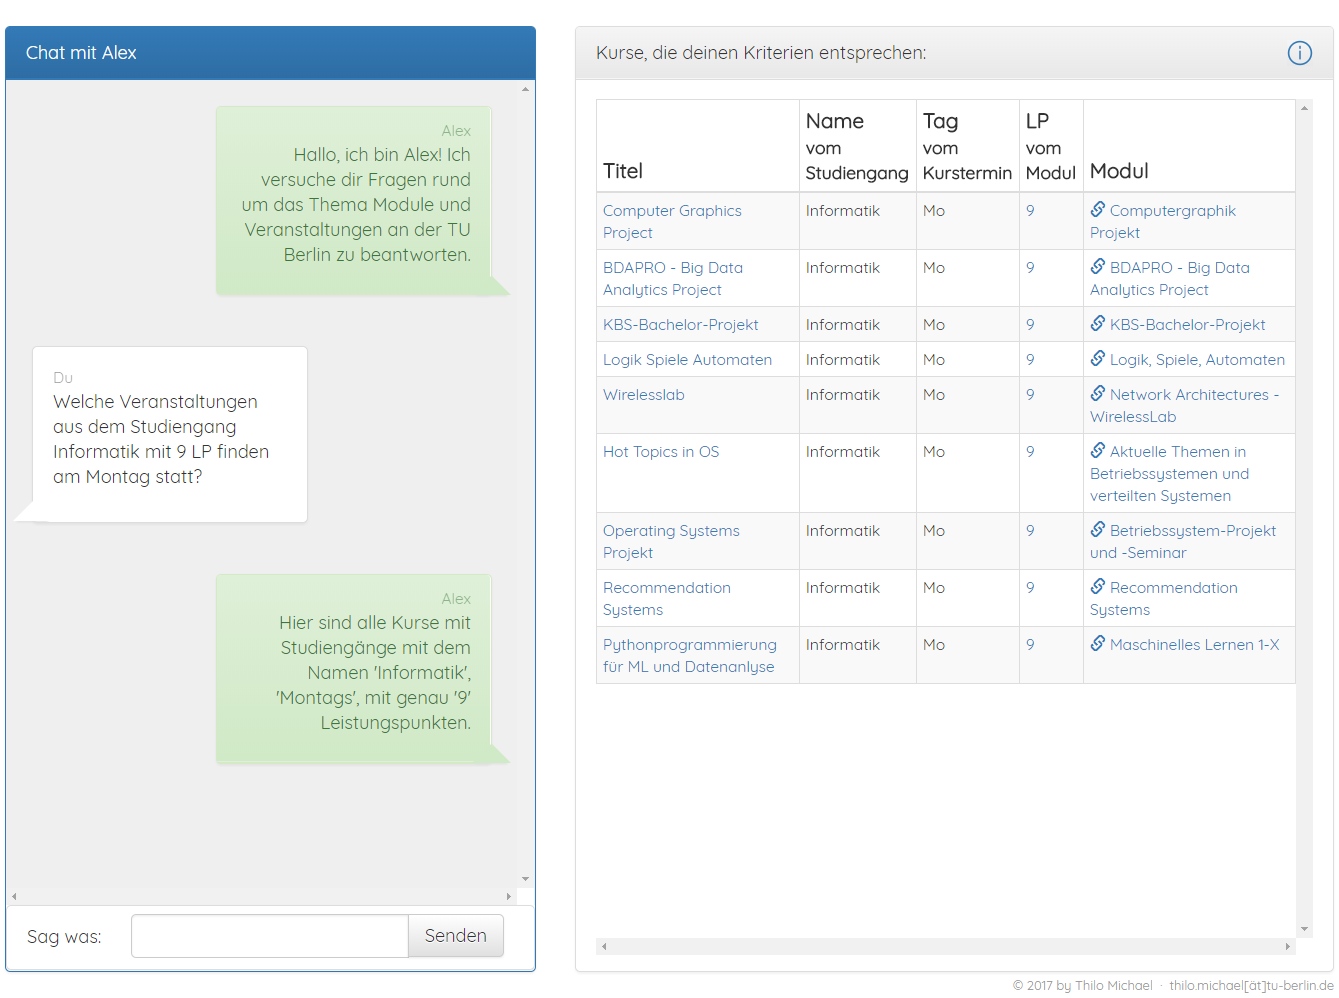
\includegraphics[width=\textwidth]{images/alex_screencapture}
	\caption[User Interface of \Alex]{The user interface of \Alex. The left section contains the conversation with the agent and a user entry field. The right section shows the result of the generated database query in tabular form.\\In this example, the user asked for all courses of the subject \i{computer science} that provide 9 ECTS and are scheduled on a Monday. The agent answered accordingly and provided a list of 9 courses that fulfill the conditions.\\This image was captured on 21st April 2018.}
	\label{f.alex_ui}
\end{figure}

\Alex\ consists of several processing modules:

\begin{itemize}
	\item The \b{tagging module} uses a hidden Markov model to calculate the parts of speech for the user input, later described in chapter \ref{c.alex.hmm}
	\item The \b{query generation module} composes actual SQL queries from the tagged output data by recognizing the requested model and the return type
	\item The \b{filter extraction module} refines the query generator and provides constraint handling for it
	\item The \b{response generation module} formulates answers for the user input using natural language by processing the generated query, the recognized model and the conversation state.
\end{itemize}

Moreover, \Alex\ provides a user interface, which utilizes web technologies and can be accessed via a web browser. Figure \ref{f.alex_ui} shows the user interface, in which the user asked a question and the agent returned the result in tabular form and answered accordingly.

The focus of this thesis lies on the tagging module, as the main objective is to replace the hidden Markov model by artificial neural networks.

\subsection{The Hidden Markov Model}\label{c.introduction.related.hmm}
The hidden Markov model (HMM) is a probabilistic finite state machine that solves general classification problems. It uses the observable output data of a system to derive hidden information from it. Among other applications, HMMs are used especially for speech recognition tasks.

The preliminary work for HMMs was done by R. L. Stratonovich. He first described conditional Markov processes in 1960 \cite{stratonovich1960}, which were used in the following years to describe simple Markov Models and later hidden Markov models (see Baum et. al. \cite{baum1966}\cite{baum1967}). The latter became a popular solution for automatic recognition of continuous speech \cite{baker1975} along with other applications, such as pattern recognition in general, the analysis of biological sequences (e.g. DNA) \cite{bishop1986} and part-of-speech tagging \cite{kupiec1992}.

\subsection{The Artificial Neural Network Model}\label{c.introduction.related.nn}
Artificial neural networks are networks that process information inspired by the biological nervous system. They consist of connected computational units, typically arranged in different layers. Such a unit (also called \i{artificial neuron}) can make calculations based on its inputs and pass the result to the neighboring units. These connections are weighted, so that the weight can be adjusted depending on the activity of the unit. Thus, a model based on the features of the input data can be created.

Following research by W. McCulloch, W. Pitts \cite{mcculloch1943} and D. Hebb \cite{shaw1986} on arithmetical learning methods, inspired by the connections of neurons in the 1940s, M. Minsky built the first neural network learning machine called SNARC (\i{Stochastic Neural Analog Reinforcement Computer)}\cite{crevier1993} in 1951.

In the late 1950s, F. Rosenblatt developed the \i{Mark I Perceptron} computer and published a theorem of convergence of the perceptron\cite{rosenblatt1958} in 1958. He coined the term \i{perceptron} for an algorithm that is able to learn the assignment of input data to different classes. The perceptron represents a simple artificial neural network initially containing one single neuron\footnote{Chapters \ref{c.postagging.fnn} and \ref{c.postagging.rnn} explain the architecture of different neural network structures in detail}. F. Rosenblatt stated that any function that is representable by the model can be learned with the proposed learning method. In 1960, B. Widrow presented the ADALINE\footnote{ADALINE is an acronym for Adaptive Linear Neuron} model of a neural network, for which input weights could already be adjusted by the learning algorithm \cite{widrow1960}.

A publication of M. Minsky and S. Papert \cite{minsky1969} from 1969 analyzed and exposed some significant limitations of the basic perceptron. They pointed out that it is impossible to learn functions without linear separability (e.g. the exclusive-or problem). Due to these limitations and the fact that the processing power of computers at the time was not sufficient for larger neural networks, research interest in artificial neural networks decreased in the following years.

In 1982, J. Hopfield presented a previously described neural network with feedback (known as \i{Hopfield network}), that was able to solve optimization problems like the \i{Traveling Salesman Problem}\footnote{The problem of the traveling salesman or round trip problem: The order of places to be visited once should be chosen in such a way that the distance covered is minimal, whereby the last place is the starting point again (round trip).}. Neural network approaches started to receive more attention again, also due to the first processors based on transistor technology (microprocessors) being introduced to the market in the early 1970s, replacing the previously used tube technology in the following years, which made computers smaller and cheaper and increased their processing capacity.

For the task of POS tagging, neural network models were now able to outperform HMM based taggers. H. Schmid created and trained a multilayer Feed-forward neural network in 1994 and was able to show that it performed better than an HMM tagger \cite{schmid1994} at that time. In 2000, Ma et. al. ran a series of comparative experiments that proved that results of a neural network tagger can be superior to those of statistical models like the HMM \cite{ma2000}.

\section{Structure of this Thesis}\label{c.introduction.structure}
This first chapter outlined the subject of natural language processing and part-of-speech tagging in general as an introduction.

The second chapter describes the structure and functionality of the already existing ACA, \Alex, with the main focus on its language model and tagging interface.

Chapter \ref{c.postagging} explains the implementation of a part-of-speech tagging system using two different neural network approaches.

The training of the language models including the retrieval of training data and tuning training parameters is described in Chapter \ref{c.training}.

Chapter \ref{c.evaluation} illustrates the evaluation of each language model with a generated test set and their comparisons.

In conclusion, \ref{c.conclusion} discusses and summarizes the evaluation results and presents an outlook on future work.

% ===================================================================================
\chapter{\Alex: Artificial Conversational Agent}\label{c.alex}
\i{Design and Implementation of an Advisory Artificial Conversational Agent} by T. Michael \cite{michael2016} provides a detailed and comprehensive description of \Alex\ as a compilation of different modules. This chapter focuses on components that are relevant for language processing and were therefore adapted during this thesis: The retrieval and processing of training data (section \ref{c.alex.data}), the hidden Markov model tagger (section \ref{c.alex.hmm}) and the tagging interface (section \ref{c.alex.tagging}).

\section{System Overview}\label{c.alex.overview}
The modular structure of \Alex\ facilitates the separation of different functions and therefore simplifies the replaceability of certain functionalities. Besides a module crawler for current data retrieval of web content for the database and a front-end interface module, \Alex\ offers a tagging module. This module enables the training of a language model as well as the assignment of tags to words of a given input sentence.

Figure \ref{f.alex.components} shows the original architecture of \Alex. The following components are part of the tagging module and are adapted or replaced (emphasized with an orange border in figure \ref{f.alex.components}) in this thesis:

\begin{itemize}
	\item The \b{HMM Training Data} is replaced by training data that was generated with improved training sentence templates (see chapter \ref{c.training.data} for a comprehensive explanation)
	\item \b{Training Data Loading and Slot Filling} are used to generate the new training data
	\item The \b{HMM Tagger} is replaced by a neural network based tagger
	\item \b{Part of Speech Tagging} of input sentences is realized by the tagging function of the new tagger
\end{itemize}

\begin{figure}[H]
	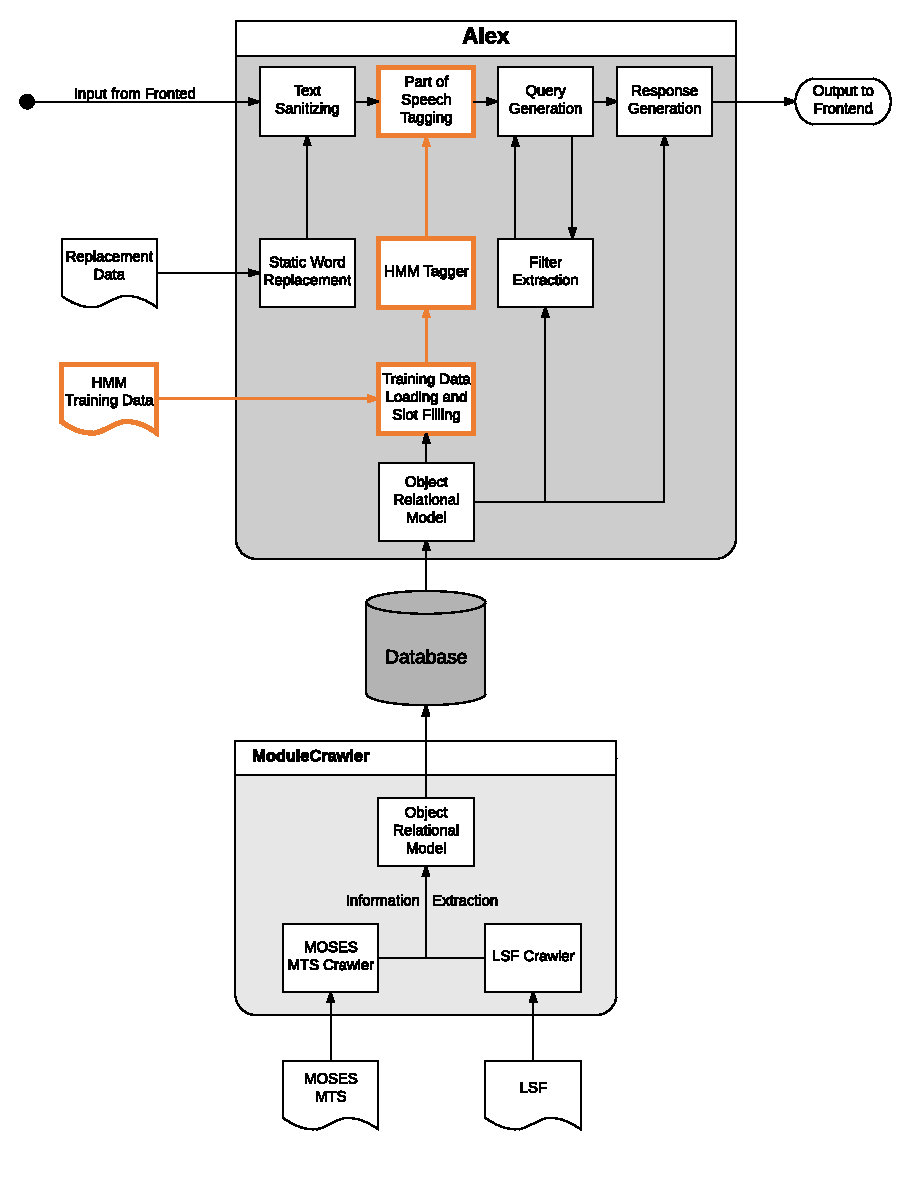
\includegraphics[width=\textwidth]{images/alex_components}
	\caption[Component Overview of \Alex]{Overview of all components of \Alex. The orange borders identify components that lie within the scope of this thesis and have been adapted or replaced. Original figure by T. Michael \cite{michael2016}}
	\label{f.alex.components}
\end{figure}

\section{Training Data}\label{c.alex.data}
In order to teach \Alex\ to assign tags to words correctly, depending on their context, appropriate training data is required. The training data for \Alex\ proposed by T. Michael consists of \tt{556,111} tagged sentences generated with \tt{72} manually created sentence templates.

A sentence template is a sentence that provides the structure of a possible tagged training sentence with proper syntax for slot filling. It consists either of special placeholders for specific data from the database (e.g. module titles), inline choices (e.g. the same sentence with each day of the week) or a marker to simply duplicate the sentence. The different slot filling forms can be combined or used multiple times in one sentence\footnote{T. Michael describes the training data structure in detail in chapter 3.4.2 of \i{Design and Implementation of an Advisory Artificial Conversational Agent} \cite{michael2016}.}.

For training the neural network models in this thesis, this slot filling mechanism is adopted and improved for the training with artificial neural networks (see chapter \ref{c.training}).

\section{The Hidden Markov Model Tagger}\label{c.alex.hmm}
As described in section \ref{c.introduction.related.hmm} \ of the introduction, the hidden Markov model (HMM) is a statistical tool that uses observable output data of a system to derive hidden information from it. Areas of application are image processing, gesture recognition and natural language processing tasks, such as speech recognition in general and part-of-speech tagging in particular.

In case of POS tagging, the observable states of the HMM represent the given sequence of words, whereas the hidden states represent the corresponding parts of speech. The HMM calculates the joint probability of the whole sequence of hidden states based on transmission and output probabilities. Subsequently, it finds the maximum probability of all possible state sequences and determines as a result, which parts of speech most likely correspond to the words of the input sequence.

Figure \ref{f.hmm_structure} illustrates an example of a state sequence with three hidden states (part of speech tags) and the observed word sequence in an HMM. The calculation of the joint probability $P$ of the word sequence in this case is shown in equation \ref{e.hmm_joint_probability}, as the product of transmission and output probabilities.

\begin{equation}
    P = p_{start}\cdot p_{out,1}\cdot p_{trans,1}\cdot p_{out,2}\cdot p_{trans,2}\cdot p_{out,3} \label{e.hmm_joint_probability}
\end{equation}

\vspace{1em}
\begin{figure}[H]
	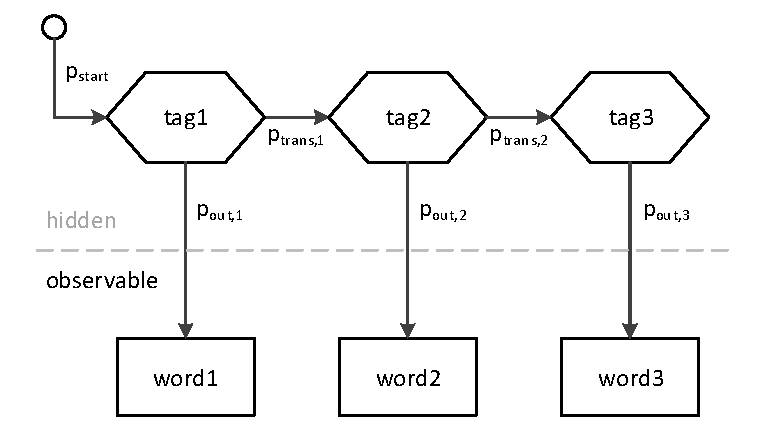
\includegraphics[width=\textwidth]{images/hmm_structure}
	\vspace{.8em}
	\caption[Structure of a Hidden Markov Model]{An example of a state sequence of three hidden states (tag1 -- tag3) and an observed sequence of three words (word1 -- word3) in a hidden Markov model. $p_{start}$ denotes the starting probability, $p_{trans}$ the transmission probabilities between hidden states and $p_{out}$ the output probabilities between a hidden state and an output.}
	\label{f.hmm_structure}
	\vspace{.8em}
\end{figure}

For the purpose of finding corresponding parts of speech to a given input sentence, an HMM is included in \Alex. According to T. Michael \cite{michael2016}, a tagging scheme was developed to extract exactly the information from user input that is needed to successfully create a database query and to return the information the user asked for. This tagging scheme was intentionally built to be domain independent, creating the opportunity to develop a version of \Alex\ for any topic based on an appropriate database and training data.

To maintain this universal applicability as well as the compatibility with other modules of \Alex, the neural network approaches presented in this thesis use the same tagging scheme \Alex\ already utilizes. For a better understanding of the evaluation results in chapter \ref{c.evaluation}, table \ref{t.tagging_scheme} gives an overview of the 6 different classes of tags that \Alex uses.

\begin{table}[H]
	\small\def\arraystretch{1.5}\begin{tabular}{ p{2mm} L{48mm} p{35mm} p{40mm} }
	\trule
	 & \textsc{Formats} & \textsc{Description} & \textsc{Example} \\
	\drule
	\tt{R} & \i{Return-tags}, describing data that is expected to be returned & \tt{R\_LIST} \newline \tt{R\_SINGLE} \newline \tt{R\_COUNT} & \i{"\b{Which} modules \dots"} \newline \i{"\b{Which} module \dots"} \newline \i{"\b{How many} modules \dots"} \\
	\mrule
	\tt{M} & \i{Model-tags}, describing the database model, e.g. \tt{M\_MTSModule} or \tt{M\_Course} & \tt{M\_[MODEL]} & \i{"Which \b{modules} \dots"} \newline \i{"Which \b{courses} \dots"} \\
	\mrule
	\tt{C} & \i{Constraint-tags}, filtering the result set, given a database model and corresponding field, e.g. \tt{C\_MTSModule:ects} & \tt{C\_[MODEL]:[FIELD]} & \i{"Modules with \b{6} ects \dots"} \\
	\mrule
	\tt{P} & \i{Property-tags}, indicating to include fields in the result set, e.g. \tt{P\_MTSModule:ects} & \tt{P\_[MODEL]:[FIELD]} & \i{"Modules with 6 \b{ects} \dots"} \\
	\mrule
	\tt{Q} & \i{Comparison-tags}, describing an equal, greater than or less than constraint & \tt{Q\_EQ} \newline \tt{Q\_LT} \newline \tt{Q\_GT} &  \i{"\dots\ with \b{exactly} 6 ects \dots"} \newline \i{"\dots\ \b{less than} 6 ects \dots"} \newline \i{"\dots\ \b{more than} 6 ects \dots"} \\
	\mrule
	\tt{X} & \i{Extra-tags}, describing words that are not relevant for the database query\tablefootnote{This can refer to words with no specific meaning (tagged with \tt{X}), words that have no meaning for the database query but for the system itself (e.g. the tag \tt{X\_HELP} for the word \i{"help"}) or words that lead to a particular constraint (such as the tag \tt{X\_Person:fullname} for the word \i{"Professor"}, leading to a name).} & \tt{X} \newline \tt{X\_[WORD]} \newline \tt{X\_[MODEL]:[FIELD]} & \i{"\b{and}"}, \i{"\b{of}"}, \i{"\b{is}"} \newline \i{"I need \b{help}"} \newline \i{"\b{Professor} John Doe"} \\
	\brule
	\end{tabular}
	\caption[Tagging Scheme Overview]{Overview of the tagging scheme used in \Alex, consisting of 6 different classes of tags with a total of 12 different formats. The examples contain \b{emphasized} words that belong to the corresponding tag formats. T. Michael \cite{michael2016} provides a detailed explanation of the tagging classes and its formats.}
	\label{t.tagging_scheme}
	\vspace{1ex}
\end{table}

\section{Tagging Interface}\label{c.alex.tagging}
As described in the previous chapter, the implementation of the tagging module of \Alex\ utilizes a hidden Markov model for part-of-speech tagging. \Alex\ uses an already existing implementation of the HMM Tagger from the Natural Language Toolkit (NLTK)\footnote{The Natural Language Toolkit is a collection of \i{Python} programming libraries for natural language processing, see \link{http://nltk.org}}, called \tt{HiddenMarkovModelTagger}.

To replace the existing tagger, a new tagger has to provide a class with two methods: \tt{train} and \tt{tag}. These methods are used to create the language model and apply it to unknown data.

The \tt{train} method creates a new instance of the tagger class, trains this class with the given training data and returns it. The training data itself must be a list of sentences, where a sentence is a list of tuples, containing each word of this sentence and its corresponding tag. The following exemplifies the structure of the training input data containing two sentences, where each word is tagged with \i{TAG}:

\lstinputlisting[language=JSON, label={l.trainingdata}]{listings/method-train.example}

The \tt{tag} method attaches a tag to each word of an input sentence, according to the previously trained language model. The input has to be an unknown sentence formatted as a simple list of words:

\lstinputlisting[language=JSON]{listings/method-tag-input.example}

The output is a corresponding list of tuples containing a word and its assigned tag:

\lstinputlisting[language=JSON]{listings/method-tag-output.example}


% ===================================================================================
\chapter{Part-of-Speech Tagging with Neural Networks}\label{c.postagging}
Chapter \ref{c.introduction.related.nn} introduced neural networks as a possible approach for POS tagging. The current chapter presents two different neural network architectures and their implementation that is later used to train and evaluate language models with the objective of comparing their POS tagging accuracy with the accuracy of the HMM tagger that \Alex\ uses.

In general, a neural network represents a mathematical function, which is able to assign specific output data to corresponding input data. This assignment is learned by processing input data whose output is known. Thus, it belongs to the category of supervised learning\footnote{\i{Supervised Learning} describes the process of gaining knowledge with the help of labeled data. Depending on the capability of the supervised learning algorithm to generalize from the given data, this knowledge can then be applied to unknown data.}.

The network itself emerges from the interconnection of nodes (the artificial neurons), that are usually arranged in different layers. Each node represents a non-linear\footnote{The non-linearity is important because linear functions cannot describe some mutual exclusive feature combinations.} activation function that calculates an output, depending on the sum of its inputs. Possible activation functions are the sigmoid function, the hyperbolic tangent or the maximum function.

The training effect is achieved by weighting the connections of the nodes and adjust these weights during training. The weights of neural networks are typically represented by real numbers. The adjustments are defined by a learning algorithm that utilizes a particular learning method. Using the initial or current weights of the network, an error (also called \i{loss}) between the prediction and the given label can be computed on the last layer (the output layer) with the help of a corresponding loss function. The training objective is to minimize the loss function of the current state of the network and adjust the weights accordingly. This can be achieved by using \i{backpropagation} with \i{stochastic gradient descent}.

The POS tagging task requires the processing of words which are represented as character strings. For easier handling, each word is mapped to an integer value (the word id).

\section{Feed-forward Neural Network Model}\label{c.postagging.fnn}
Feed-forward neural networks are a common type of ANNs, that consist of an input and an output layer with one or more hidden layers in between. An FNN propagates information through the network only in the forward direction, from the input to the output layer.

\subsection{Architecture}\label{c.postagging.fnn.architecture}
The FNN architecture that is used in this thesis is shown in figure \ref{f.fnn.structure}. The current word and the configured number of preceding words are each converted into word embeddings. These embeddings are reshaped to one vector, called the feature vector, which serves as the input layer for the neural network. The FNN contains one hidden layer, which is connected to the input layer with weight matrix \tt{V}. The output layer represents the set of existing POS tags and is connected to the hidden layer with weight matrix \tt{W}.

For each word of every sentence of the training corpus, a feature vector is built and the data is sequentially propagated to both the hidden and the output layer, predicting a POS tag for the current word and calculating the current loss and accuracy. After propagating the error back to adjust the weights and reduce the loss, the next training step is executed.

\begin{figure}[ht]
	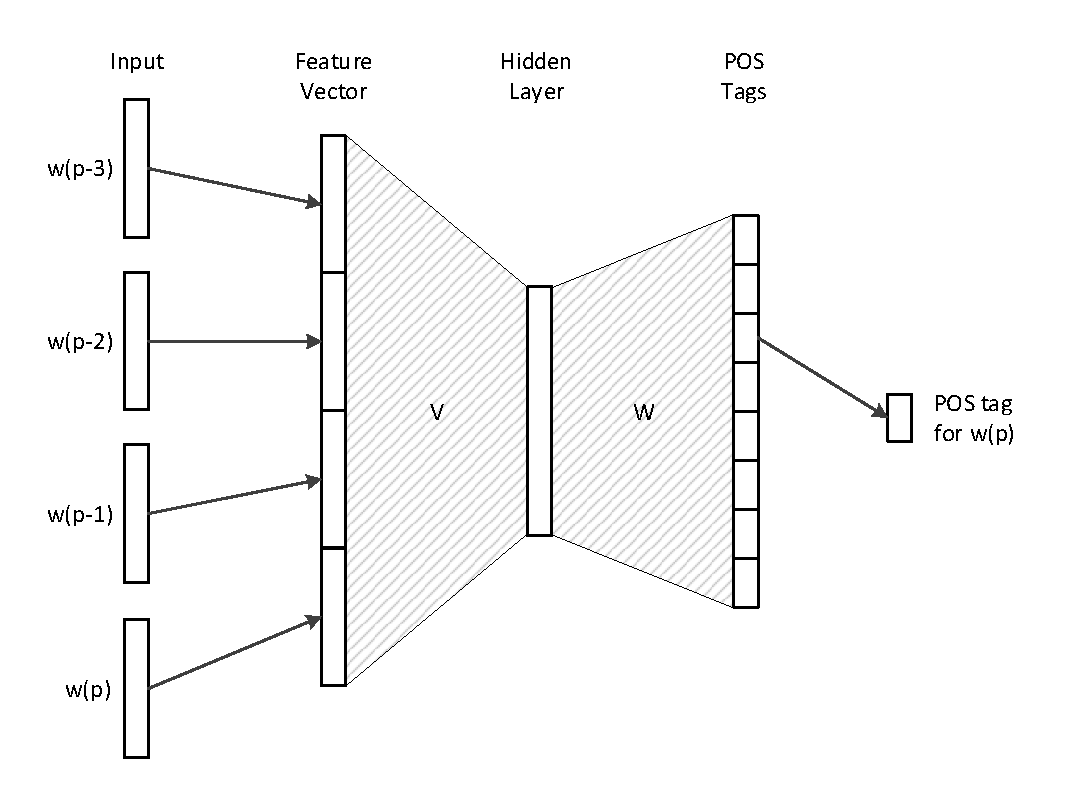
\includegraphics[width=\textwidth]{images/fnn_structure}
	\caption[Structure of a Feed-forward Neural Network]{The structure of a feed-forward neural network. The feature vector is built by the embeddings of the corresponding input word at position \tt{p} and by its \tt{3} preceding words (the number of predecessors may vary, of course). \tt{V} and \tt{W} are weight matrices with respective matrix dimensions of $\textsf{feature vector size} \times \textsf{hidden layer size}$ for \tt{V} and $\textsf{hidden layer size} \times \textsf{number of POS tags}$ for \tt{W}.}
	\label{f.fnn.structure}
\end{figure}

\subsection{Implementation}\label{c.postagging.fnn.implementation}
To implement the presented FNN architecture, the open source machine learning framework \i{TensorFlow}\footnote{TensorFlow is a library written in Python, that is utilized for high performance numerical computations especially for the area of machine learning. In this thesis, TensorFlow version 1.8 is used.\\See the official TensorFlow website: \link{https://www.tensorflow.org}} is used. In the following descriptions, all functions starting with \tt{tf} are functions from the TensorFlow library.

The nodes of the input layer are populated by the feature vector. To create the feature vector, an embedding matrix with the dimensions of $\textsf{vocabulary size} \times \textsf{embedding size}$ is created and initially filled with random normal distributed values\footnote{The generated values follow a normal distribution with mean of 0 and standard deviation of 0.1, except that values whose magnitude is more than two standard deviations from the mean are dropped (truncated) and re-picked. See the TensorFlow documentation.}, using the \tt{tf.truncated\_normal()} function. This matrix is used to retrieve the vectors for the current word and its predecessors via \tt{tf.nn.embedding\_lookup} and reshape them to one single vector, the feature vector. Figure \ref{f.fnn.feature} illustrates the creation of the feature vector.

\begin{figure}[ht]
	\vspace{1.5em}
	\hspace{-1.5em}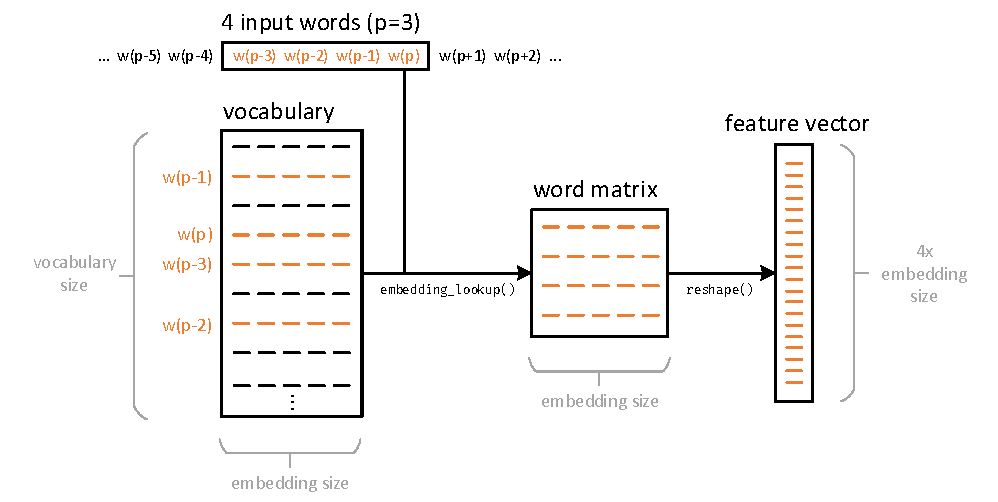
\includegraphics[width=1.1\textwidth]{images/feature_vector}
	\caption[Creation of the feature vector]{An example of the creation of a feature vector for the FNN using \tt{3} preceding words and the current word.}
	\label{f.fnn.feature}
	\vspace{.5em}
\end{figure}

The hidden layer nodes are also initialized with random normal distributed values. Their outputs are computed with the rectified linear activation function (the \i{rectifier}), utilizing the \tt{tf.nn.relu()} function. These nodes are therefore also called \i{rectified linear units} (RELUs).

Finally, the values for the output layer (the logits) are computed using a matrix multiplication of the outputs of the RELUs and the weight matrix \tt{W} using the \tt{tf.matmul()} function. Subsequently, the loss can be calculated by computing the sparse softmax cross entropy between input labels and logits, using the \tt{tf.nn.sparse\_softmax\_cross\_entropy\_with\_logits()} function.

The predictions are calculated with the \tt{tf.argmax()} function, that reduces the logits to the largest value, which represents the predicted POS tag. The function \tt{tf.train.AdamOptimizer()}\footnote{The Adam algorithm is an optimizer that was proposed by D. Kingma et. al. in 2014 \cite{kingma2014}. It provides a computationally efficient gradient-based optimization of stochastic objective functions.} enables backpropagation with stochastic gradient descent to optimize the computations and results during training.


\section{Recurrent Neural Network Model}\label{c.postagging.rnn}
Similar to FNNs, recurrent neural networks (RNNs) also consist of an input, a hidden and an output layer. The main difference is that information is not only propagated forward linearly, but that information from previous training steps are also taken into account in RNNs.

\subsection{Architecture}\label{c.postagging.rnn.architecture}
Figure \ref{f.rnn.structure} illustrates the architecture of an RNN, which was implemented for this thesis. Unlike the FNN, the RNN only uses word ids as input features and does not utilize word embeddings. It contains one hidden layer, which is populated with the current input word on the one hand and by the output of the hidden layer of a previous training step on the other hand. This makes the RNN capable of memorizing information from the past. This capability can also be described as a long short-term memory (\i{LSTM}), emphasized in orange in figure \ref{f.rnn.structure}. The output layer represents the set of existing POS tags and is connected to the hidden layer with weight matrix
\tt{W}.

Each word of every sentence of the training corpus represents an input feature, which is propagated to the hidden and the output layer together with information from previous training steps. Similar to the processing of FNNs, the POS tag is predicted for the current word and the current loss and accuracy are calculated. After propagating the error back to adjust the weights and reduce the loss, the next training step is executed, taking the current training step into account.

\begin{figure}[ht]
	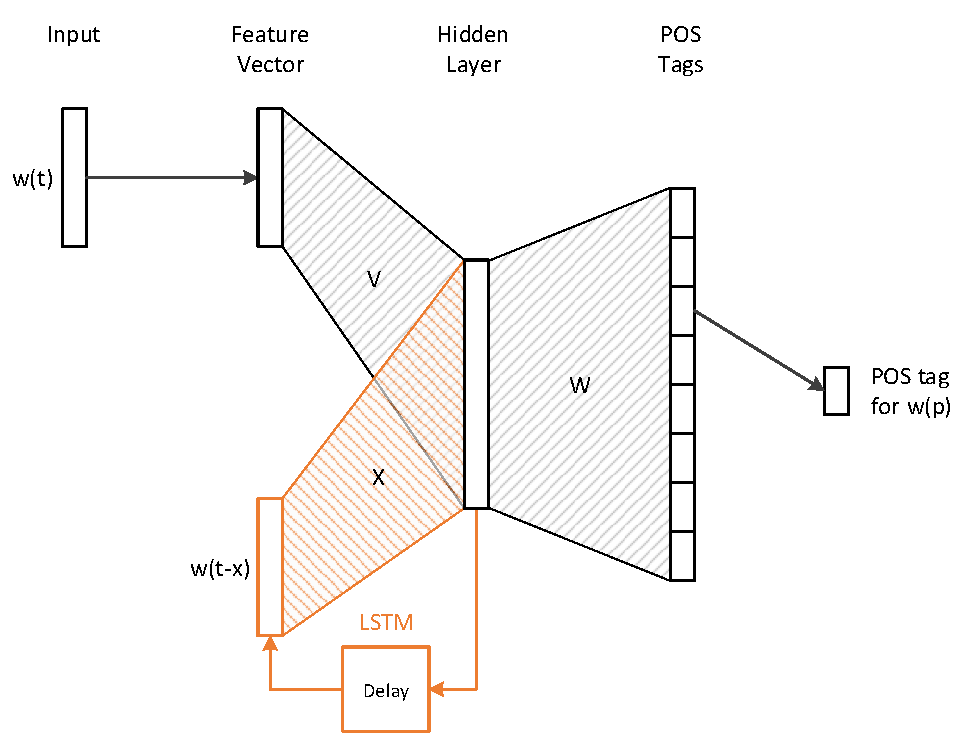
\includegraphics[width=\textwidth]{images/rnn_structure}
	\caption[Structure of a Recurrent Neural Network]{The structure of a recurrent neural network. The feature vector is the initial vector of the corresponding input word at time \tt{t}. The output of the hidden layer from previously trained words (here at time \tt{t-x}) is populated back into the same hidden layer for the current word. \tt{V}, \tt{X} and \tt{W} are weight matrices with respective matrix dimensions of $\textsf{feature vector size} \times \textsf{hidden layer size}$ for \tt{V}, $\textsf{hidden layer size} \times \textsf{hidden layer size}$ for \tt{X} and $\textsf{hidden layer size} \times \textsf{number of POS tags}$ for \tt{W}.}
	\label{f.rnn.structure}
\end{figure}

\subsection{Implementation}\label{c.postagging.rnn.implementation}
The implementation of the proposed RNN architecture utilizes the TensorFlow library as well. Besides the word id of the current word, the input layer has an additional dimension describing the number of past training steps that are considered for the current training step.

The hidden layer is built using \tt{tf.nn.rnn\_cell.LSTMCell()}\footnote{This function uses an implementation proposed by S. Hochreiter et. al. in 1997 \cite{hochreiter1997}.}, a function that creates a long short-term memory (LSTM) cell for recurrent networks which is then used in \tt{tf.nn.dynamic\_rnn()} to compute the logits for the output layer.

Loss, predictions and accuracy are implemented in a similar way as in the FNN. In addition, the same optimizer is used.

% ===================================================================================
\chapter{Training of Language Models}\label{c.training}
An optimal language model using the neural network approach proposed in this thesis, requires as much annotated training data as possible. The following sections describe the generation of tagged training data and the training of different language models, due to parameter variation, based on this generated training corpus.

\section{Training Data Corpus}\label{c.training.data}
To create a training corpus with tagged sentences, the already existing sentence template set of \Alex\ is used as the basis for an improved and extended template set. In addition, a log of user input data\footnote{The log data that was available for this thesis started on 30th of August, 2017 until 27th of April, 2018 and contained \tt{1293} entries of user input.} provides useful information on possible input sentences, that are not yet considered in the template set.

As described in chapter \ref{c.alex.data}, the HMM tagger of \Alex\ uses \tt{72} sentence templates to generate annotated training data. However, the distribution of the generated sentences is highly unbalanced. Due to the combination of placeholders for different database fields and models, which are semantically meaningless, a huge number of training sentences exist that are only partially suitable for training.

An analysis of the generated training corpus that was used to train the HMM tagger showed that one single template of the \tt{72} sentence templates created more than \tt{84\%} of the whole training corpus. This sentence template is the following\footnote{The corresponding English translation of this sentence template is: \i{Which modules are held by Professor <firstname> <lastname>}}:

\vbox{\begin{Verbatim}[fontsize=\scriptsize]
Welche   Module  werden von   Prof   {Person:firstname} {Person:lastname} angeboten
\end{Verbatim}
\vspace{-6mm}
{\color{gray}\begin{Verbatim}[fontsize=\scriptsize]
R_LIST M_MTSModule  X    X  X_Person C_Person:fullname  C_Person:fullname     X
\end{Verbatim}
}}

It combines all first names and all last names of each existing person in the database, leading to a huge number of name combinations that do not exist.

Another example is the combination of study program degrees and program names. This combination exists in \tt{5} of the \tt{72} sentence templates, i.e. all degrees are assigned to all study programs \tt{5} times, although not every combination exists in reality. The following is an example of one of these sentence templates\footnote{The corresponding English translation of this sentence template is: \i{Which modules can I attend to in <program-degree> <program-name>}}:

\vbox{\begin{Verbatim}[fontsize=\scriptsize]
Welche   Module    kann ich  im  {Program:degree}  {Program:name} belegen
\end{Verbatim}
\vspace{-6mm}
{\color{gray}\begin{Verbatim}[fontsize=\scriptsize]
R_LIST M_MTSModule  X    X   X   C_Program:degree  C_Program:name    X
\end{Verbatim}
}}

To address this issue, the following adjustments were made for the new template set were made:

\begin{itemize}
	\item Because the number of occurrences is very low in the log database, the slot \tt{\{Person:firstname\}} was removed completely from the sentence template, which limits the user input to last names only\footnote{This might seem like a degradation but is justified by the fact, that only \tt{3} of \tt{1293} log entries (\tt{0.2\%}) even contained a first name, always followed by the last name. In this specific use case, where all persons are professors and lecturers, using the last name only is a reasonable approach.}.
	\item The slot \tt{\{Program:degree\}} was partly replaced by the inline choice \tt{(bachelor|master|diplom)}, which included the main terms requested in the logs.
\end{itemize}

Furthermore, wording referring to linking words and actions, which occurs in the logs, was improved with the help of inline choices. The following table shows an excerpt of those improvements, comparing the previous and the new sentence template:

\begin{table}[H]
	\small\def\arraystretch{1.5}\begin{tabular}{ L{43mm} L{43mm} p{43mm} }
	\trule
	\textsc{Previous Template} & \textsc{New Template} & \multicolumn{1}{L{43mm}}{\textsc{English Equivalent}} \\
	\drule
	Alle Module \b{vom} \{Program:degree\} \{Program:name\} & Alle Module \b{(vom|von|in|im)} \{Program:degree\} \{Program:name\} & \multicolumn{1}{L{43mm}}{\i{All modules \b{(of|in)} \{Program:degree\} \{Program:name\} }} \\
	\mrule
	Welche Module werden von Prof \{Person:firstname\} \{Person:lastname\} \b{angeboten} & Welche Module werden von Professor \{Person:lastname\} \b{(unterrichtet| angeboten|gehalten)} & \multicolumn{1}{L{43mm}}{\i{Which modules are \b{(taught|offered|held)} by Professor \{Person:lastname\} }} \\
	\mrule
	\b{Wieviele} LP \b{hat} das Modul \{MTSModule:title\} & \b{(Wieviele|Wieviel)} LP \b{(hat|bringt)} das Modul \{MTSModule:title\} & \multicolumn{1}{L{43mm}}{\i{\b{How many} ects does the module \{MTSModule:title\} \b{(have|yield)} }} \\
	\mrule
	\b{Informationen} \b{zu} Modul {MTSModule:title} & \b{(Informationen|Details| Mehr)} \b{(zu|zum)} Modul \{MTSModule:title\} & \multicolumn{1}{L{43mm}}{\i{\b{(Information|details| more)} \b{of} the module \{MTSModule:title\} }} \\
	\brule
	\end{tabular}
	\caption[Sentence Template Improvements]{An excerpt of the extension and improvement of the sentence templates by using inline choices. The last column provides the corresponding English translation for the new sentence template.}
	\label{t.improved_sentence_templates}
	\vspace{1em}
\end{table}

All in all, the new set of sentence templates contains \tt{36} templates, which are exactly the same as in the old set, \tt{29} templates that were slightly modified or extended while maintaining the same tag sequence and \tt{35} new sentence templates. The latter were created according to a sentence structure that was found in the logs but not in the previous template set. Therefore, the new set contains a total of \tt{100} sentence templates (including single word templates) and can be found in the appendix \ref{c.appendix.sentencetemplates}.

The resulting training data corpus used in this thesis contains \tt{218.700} tagged sentences consisting of \tt{2.038.490} words, with a vocabulary of \tt{9141} words.

\section{Parameter Tuning}\label{c.training.tuning}
In order to achieve better evaluation results and therefore more words that are tagged correctly, several training parameters are changed. To see the effect of the training parameters on the accuracy of the resulting language model, one parameter was altered while keeping all other parameters constant.

For the training of the FNN models, the following \tt{4} parameters were considered:

\begin{itemize}
	\item \b{Number of past words} (\tt{\b{p}}) specifies how many preceding words should be considered for the training of the current word
	\item \b{Embedding size} (\tt{\b{e}}) describes the dimension of the word embeddings that were created for each word of the vocabulary during training
	\item \b{Hidden layer size} (\tt{\b{s}}) characterizes the dimension of the hidden layer, i.e. the number of neurons that constitute the hidden layer
	\item \b{Number of training epochs} (\tt{\b{n}}) indicates how often the whole training corpus is processed during training
	\item \b{Activation function} (\tt{\b{a}}) ...
\end{itemize}

Based on these \tt{5} parameters, table \ref{t.training.tuning.fnn} shows different parameter combinations. The emphasized cells show the respective parameter that is variable. The first \tt{4} training groups represent the basic training process to demonstrate the effect of each parameter in general. The subsequent training groups included additional parameter combinations, taking into account the evaluation results of the first training groups.

The resulting number of models is \tt{99}; however, due to an overlap in configurations of the training groups, the total number of distinct models to be trained with the FNN is \tt{??}.

\begin{table}[H]
	\vspace{2em}
	\centering\small\def\arraystretch{1.5}\begin{tabular}{ c c c c c c }
	\trule
	\tt{p} & \tt{e} & \tt{s} & \tt{n} & \tt{a} & \textsc{Models} \\
	\drule
	\cellcolor{orange}\color{white}\b{\tt{0}--\tt{12}} & \tt{50} & \tt{100} & \tt{1} & \tt{relu} & \tt{13} \\
	\mrule
	\tt{1} & \cellcolor{orange}\color{white}\b{\tt{1}, \tt{5}, \tt{10}, \tt{25}} & \tt{100} & \tt{1} & \tt{relu} & \tt{4} \\
	\mrule
	\tt{1} & \cellcolor{orange}\color{white}\b{\tt{50}--\tt{700}\tablefootnote{With a step size of \tt{50}\label{fifty}}} & \tt{100} & \tt{1} & \tt{relu} & \tt{14} \\
	\mrule
	\tt{1} & \tt{50} & \cellcolor{orange}\color{white}\b{\tt{10}, \tt{25}} & \tt{1} & \tt{relu} & \tt{2} \\
	\mrule
	\tt{1} & \tt{50} & \cellcolor{orange}\color{white}\b{\tt{50}--\tt{1000}\footref{fifty}} & \tt{1} & \tt{relu} & \tt{20} \\
	\mrule
	\tt{1} & \tt{50} & \tt{100} & \cellcolor{orange}\color{white}\b{\tt{1}, \tt{5}, \tt{10}} & \tt{relu} & \tt{3} \\
	\mrule
	\tt{1} & \tt{50} & \tt{100} & \cellcolor{orange}\color{white}\b{\tt{20}--\tt{140}\tablefootnote{With a step size of \tt{20}}} & \tt{relu} & \tt{7} \\
	\mrule
	\tt{1} & \tt{250} & \tt{350} & \tt{1} & \cellcolor{orange}\color{white}\b{\tt{relu}, \tt{[...]}\tablefootnote{The following activation functions were considered: \ftt{relu}, \ftt{relu6}, \ftt{elu}, \ftt{sigmoid}, \ftt{tanh}, \ftt{selu}, \ftt{softplus}, \ftt{softsign}}} & \tt{8} \\
	\srule
	\tt{1} & \cellcolor{orange}\color{white}\b{\tt{200}--\tt{600}\footref{fifty}} & \tt{350} & \tt{1} & \tt{relu} & \tt{9} \\
	\mrule
	\tt{1} & \tt{250} & \cellcolor{orange}\color{white}\b{\tt{200}--\tt{600}\footref{fifty}} & \tt{1} & \tt{relu} & \tt{9} \\
	\mrule
	\tt{1} & \cellcolor{orange}\color{white}\b{\tt{50}--\tt{500}\footref{fifty}} & \cellcolor{orange}\color{white}\b{\tt{50}--\tt{500}\footref{fifty}} & \tt{5} & \tt{relu} & \tt{10} \\
	\brule
	\end{tabular}
	\caption[Parameter combinations of FNN Models]{The parameter configuration for training the FNN models. The rows represent the training groups with the corresponding variable parameter (orange cells), while the columns represent the single training parameters (\tt{\b{p}} - number of past words, \tt{\b{e}} - embedding size, \tt{\b{s}} - hidden layer size, \tt{\b{n}} - number of training epochs, \tt{\b{a}} - activation function). The last column shows the resulting number of models for each training group.}
	\label{t.training.tuning.fnn}
	\vspace{1em}
\end{table}

For the training of the RNN models, the following \tt{3} parameters were considered:

\begin{itemize}
	\item \b{Number of time steps} (\tt{\b{t}}) specifies how many past training steps should be considered for the training of the current word
	\item \b{Hidden layer size} (\tt{\b{s}}) characterizes the dimension of the hidden layer, i.e. the number of neurons that constitute the hidden layer
	\item \b{Number of training epochs} (\tt{\b{n}}) indicates how often the whole training corpus is processed during training
\end{itemize}

Based on these \tt{3} parameters, table \ref{t.training.tuning.rnn} shows different parameter combinations. The emphasized cells show the respective parameter that is variable. The resulting number of models is \tt{18}; however, due to an overlap in configurations of the training groups, the total number of models to be trained with the RNN is \tt{16}.

\begin{table}[ht]
	\vspace{2em}
	\centering\small\def\arraystretch{1.5}\begin{tabular}{ c c c c c }
	\trule
	\tt{t} & \tt{s} & \tt{n} & \textsc{Models} \\
	\drule
	\cellcolor{orange}\color{white}\b{\tt{0}--\tt{10}} & \tt{50} & \tt{10} & \tt{10} \\
	\mrule
	\tt{1} & \cellcolor{orange}\color{white}\b{\tt{10}, \tt{25}, \tt{50}, \tt{100}} & \tt{10} & \tt{4} \\
	\mrule
	\tt{1} & \tt{50} & \cellcolor{orange}\color{white}\b{\tt{1}, \tt{5}, \tt{10}, \tt{20}} & \tt{4} \\
	\brule
	\end{tabular}
	\caption[Parameter combinations of RNN Models]{The parameter configuration for the training of RNN models. The rows represent the training groups with the corresponding variable parameter (orange cells), while the columns represent the single training parameters (\tt{\b{t}} (number of time steps), \tt{\b{s}} (hidden layer size), \tt{\b{n}} (number of training epochs)). The last column shows the resulting number of models for each training group.}
	\label{t.training.tuning.rnn}
\end{table}

% ===================================================================================
\chapter{Evaluation and Comparison}\label{c.evaluation}
After a short description of how the evaluation tests were created, this chapter provides the evaluation results of all models that were trained using the variation of training parameters previously described. Additionally, for each training group, the evaluation results are presented and the three different architectures (FNN, RNN and HMM) are compared.

\section{Test Design}\label{c.evaluation.test}
To evaluate the trained language models, two test sets were designed: a test set containing a selection of tagged sentences that actually exist in the training corpus (here called the \i{known test}) and a test set, for which the structure of the sentences in the known test was modified in a way that it remains semantically meaningful but does not occur in the training corpus (called the \i{unknown test}). The unknown test deliberately contains words, which do not exist in the vocabulary of the training corpus in order to assess how the model handles completely unknown data.

The sentences are divided into different topics to cover a wide range of possible input data. A balanced number of sentences was included in the different areas to ensure that the evaluation result does not depend on only one or two topics.

Tables \ref{t.evaluation_topics_known} and \ref{t.evaluation_topics_unknown} show the different topics represented in the known and the unknown test set, the respective number of evaluation sentences and an example sentence to illustrate each topic. Both test sets combined include a total number of \tt{1058} tagged test sentences, consisting of \tt{7678} word-tag tuples.

\begin{table}[!ht]
	\centering\small\def\arraystretch{1.5}\begin{tabular}{ p{18mm} c L{95mm} }
	\trule
	\textsc{Topic} & \textsc{Sentences} & \multicolumn{1}{L{95mm}}{\textsc{Example}} \\
	\drule
	ECTS & \tt{44} & \multicolumn{1}{L{95mm}}{\i{Which modules have 6 ECTS}} \\
	\mrule
	Time & \tt{60} & \multicolumn{1}{L{95mm}}{\i{Which courses are on Tuesday}} \\
	\mrule
	Faculty & \tt{56} & \multicolumn{1}{L{95mm}}{\i{All modules of faculty 4}} \\
	\mrule
	Participants & \tt{54} & \multicolumn{1}{L{95mm}}{\i{Which courses are limited to 30 participants}} \\
	\mrule
	Persons & \tt{61} & \multicolumn{1}{L{95mm}}{\i{Which courses are taught by Professor Martinelli}} \\
	\mrule
	Program & \tt{60} & \multicolumn{1}{L{95mm}}{\i{I'm searching for all modules of the computer science program }} \\
	\mrule
	Modules & \tt{80} & \multicolumn{1}{L{95mm}}{\i{Modules with the title Cognitive Algorithms}} \\
	\mrule
	Chair & \tt{50} & \multicolumn{1}{L{95mm}}{\i{All modules of institute Media Science}} \\
	\mrule
	Exam & \tt{32} & \multicolumn{1}{L{95mm}}{\i{Courses with Group Lecture as examination}} \\
	\mrule
	Courses & \tt{45} & \multicolumn{1}{L{95mm}}{\i{When does Internet Security take place}} \\
	\mrule
	Locations & \tt{42} & \multicolumn{1}{L{95mm}}{\i{All courses in room Mainbuilding H 1012}} \\
	\bottomrule
	 & \tt{584} & \\
	\end{tabular}
	\vspace{3mm}
	\caption[Evaluation Topics using the Known Test Set]{The evaluation topics, the number of tagged test sentences and an example sentence for each topic in the known test set. It contains a total of \tt{584} tagged sentences, consisting of \tt{4009} word-tag tuples.}
	\label{t.evaluation_topics_known}
	\vspace{1em}
\end{table}

\begin{table}[!ht]
	\centering\small\def\arraystretch{1.5}\begin{tabular}{ p{18mm} c L{95mm} }
	\trule
	\textsc{Topic} & \textsc{Sentences} & \multicolumn{1}{L{95mm}}{\textsc{Example}} \\
	\drule
	ECTS & \tt{44} & \multicolumn{1}{L{95mm}}{\i{All modules with 6 ECTS}} \\
	\mrule
	Time & \tt{55} & \multicolumn{1}{L{95mm}}{\i{Courses that take place on Tuesday}} \\
	\mrule
	Faculty & \tt{56} & \multicolumn{1}{L{95mm}}{\i{Show all modules of faculty 4 to me}} \\
	\mrule
	Participants & \tt{54} & \multicolumn{1}{L{95mm}}{\i{List all courses that have a limitation of 30 participants}} \\
	\mrule
	Persons & \tt{58} & \multicolumn{1}{L{95mm}}{\i{Show all courses that are taught by Professor Martinelli}} \\
	\mrule
	Program & \tt{10} & \multicolumn{1}{L{95mm}}{\i{Show all modules of computer science }} \\
	\mrule
	Modules & \tt{60} & \multicolumn{1}{L{95mm}}{\i{Show information about the module Cognitive Algorithms}} \\
	\mrule
	Chair & \tt{20} & \multicolumn{1}{L{95mm}}{\i{All modules that the institute Media Science offers}} \\
	\mrule
	Exam & \tt{45} & \multicolumn{1}{L{95mm}}{\i{Show me all courses that have Group Lecture as examination}} \\
	\mrule
	Courses & \tt{30} & \multicolumn{1}{L{95mm}}{\i{The date of the first meeting of Internet Security }} \\
	\mrule
	Locations & \tt{42} & \multicolumn{1}{L{95mm}}{\i{All courses in auditorium Mainbuilding H 1012}} \\
	\bottomrule
	 & \tt{474} & \\
	\end{tabular}
	\vspace{3mm}
	\caption[Evaluation Topics using the Unknown Test Set]{The evaluation topics, the number of tagged test sentences and an example sentence for each topic in the unknown test set. It contains a total of \tt{474} tagged sentences, consisting of \tt{3669} word-tag tuples.}
	\label{t.evaluation_topics_unknown}
\end{table}

The number of correctly tagged words serves as a measure of accuracy for the respective language model. This includes unrecognized words (words that did not occur in the training corpus) that are still tagged correctly. The proportion of correctly tagged words can then be compared for both test sets for each language model.

In addition, the conformity of the language models with the labeled test data is measured by using Cohen's Kappa ($\kappa$)\footnote{Cohen's Kappa is a measurement of the agreement of two raters referring to a given set of categories (in this thesis the set of tags). It was proposed by J. Cohen in 1960 \cite{cohen1960} and considers the possibility of agreement by chance.}. The definition of Cohen's Kappa is given in equation \ref{e.kappa}.

\begin{equation}
\kappa = \frac{p_o - p_c}{1 - p_c} \label{e.kappa}
\end{equation}

$p_o$ represents the measured agreement and $p_c$ the randomly expected agreement. Most values are between the perfect agreement ($\kappa = 1$) and an agreement only by chance ($\kappa = 0$). Values lower than zero are interpreted as an agreement that is even worse than an agreement by chance. There are different interpretations of the level of agreement for the different values of $\kappa$. Table \ref{t.evaluation.kappa} presents an interpretation based on a proposal of J. Landis et. al. \cite{landis1977} is used in this thesis.

\begin{table}[!ht]
	\centering\small\def\arraystretch{1.5}\begin{tabular}{ r l }
	\trule
	\textsc{Cohen's Kappa} & \textsc{Interpretation} \\
	\srule
	$\kappa \leq 0.2$ \ \ & Poor agreement \\
	\mrule
	$0.2 < \kappa \leq 0.4$ \ \ & Fair agreement \\
	\mrule
	$0.4 < \kappa \leq 0.6$ \ \ & Moderate agreement \\
	\mrule
	$0.6 < \kappa \leq 0.8$ \ \ & Good agreement \\
	\mrule
	$0.8 < \kappa \leq 1.0$ \ \ & Very good agreement \\
	\brule
	\end{tabular}
	\vspace{.8em}
	\caption[Interpretation of Cohen's Kappa]{The interpretation of Cohen's Kappa for different levels of agreement of two raters.}
	\label{t.evaluation.kappa}
\end{table}

\section{Evaluation Results}\label{c.evaluation.results}
After introducing the test sets and the evaluation methodology, all training groups were evaluated according to the parameter configuration presented in chapter \ref{c.training.tuning}. The following sections show the evaluation results of the different architectures for each test set.

\subsection{Feed-Forward Neural Network Models}\label{c.evaluation.results.fnn}
...

\begin{figure}[H]
	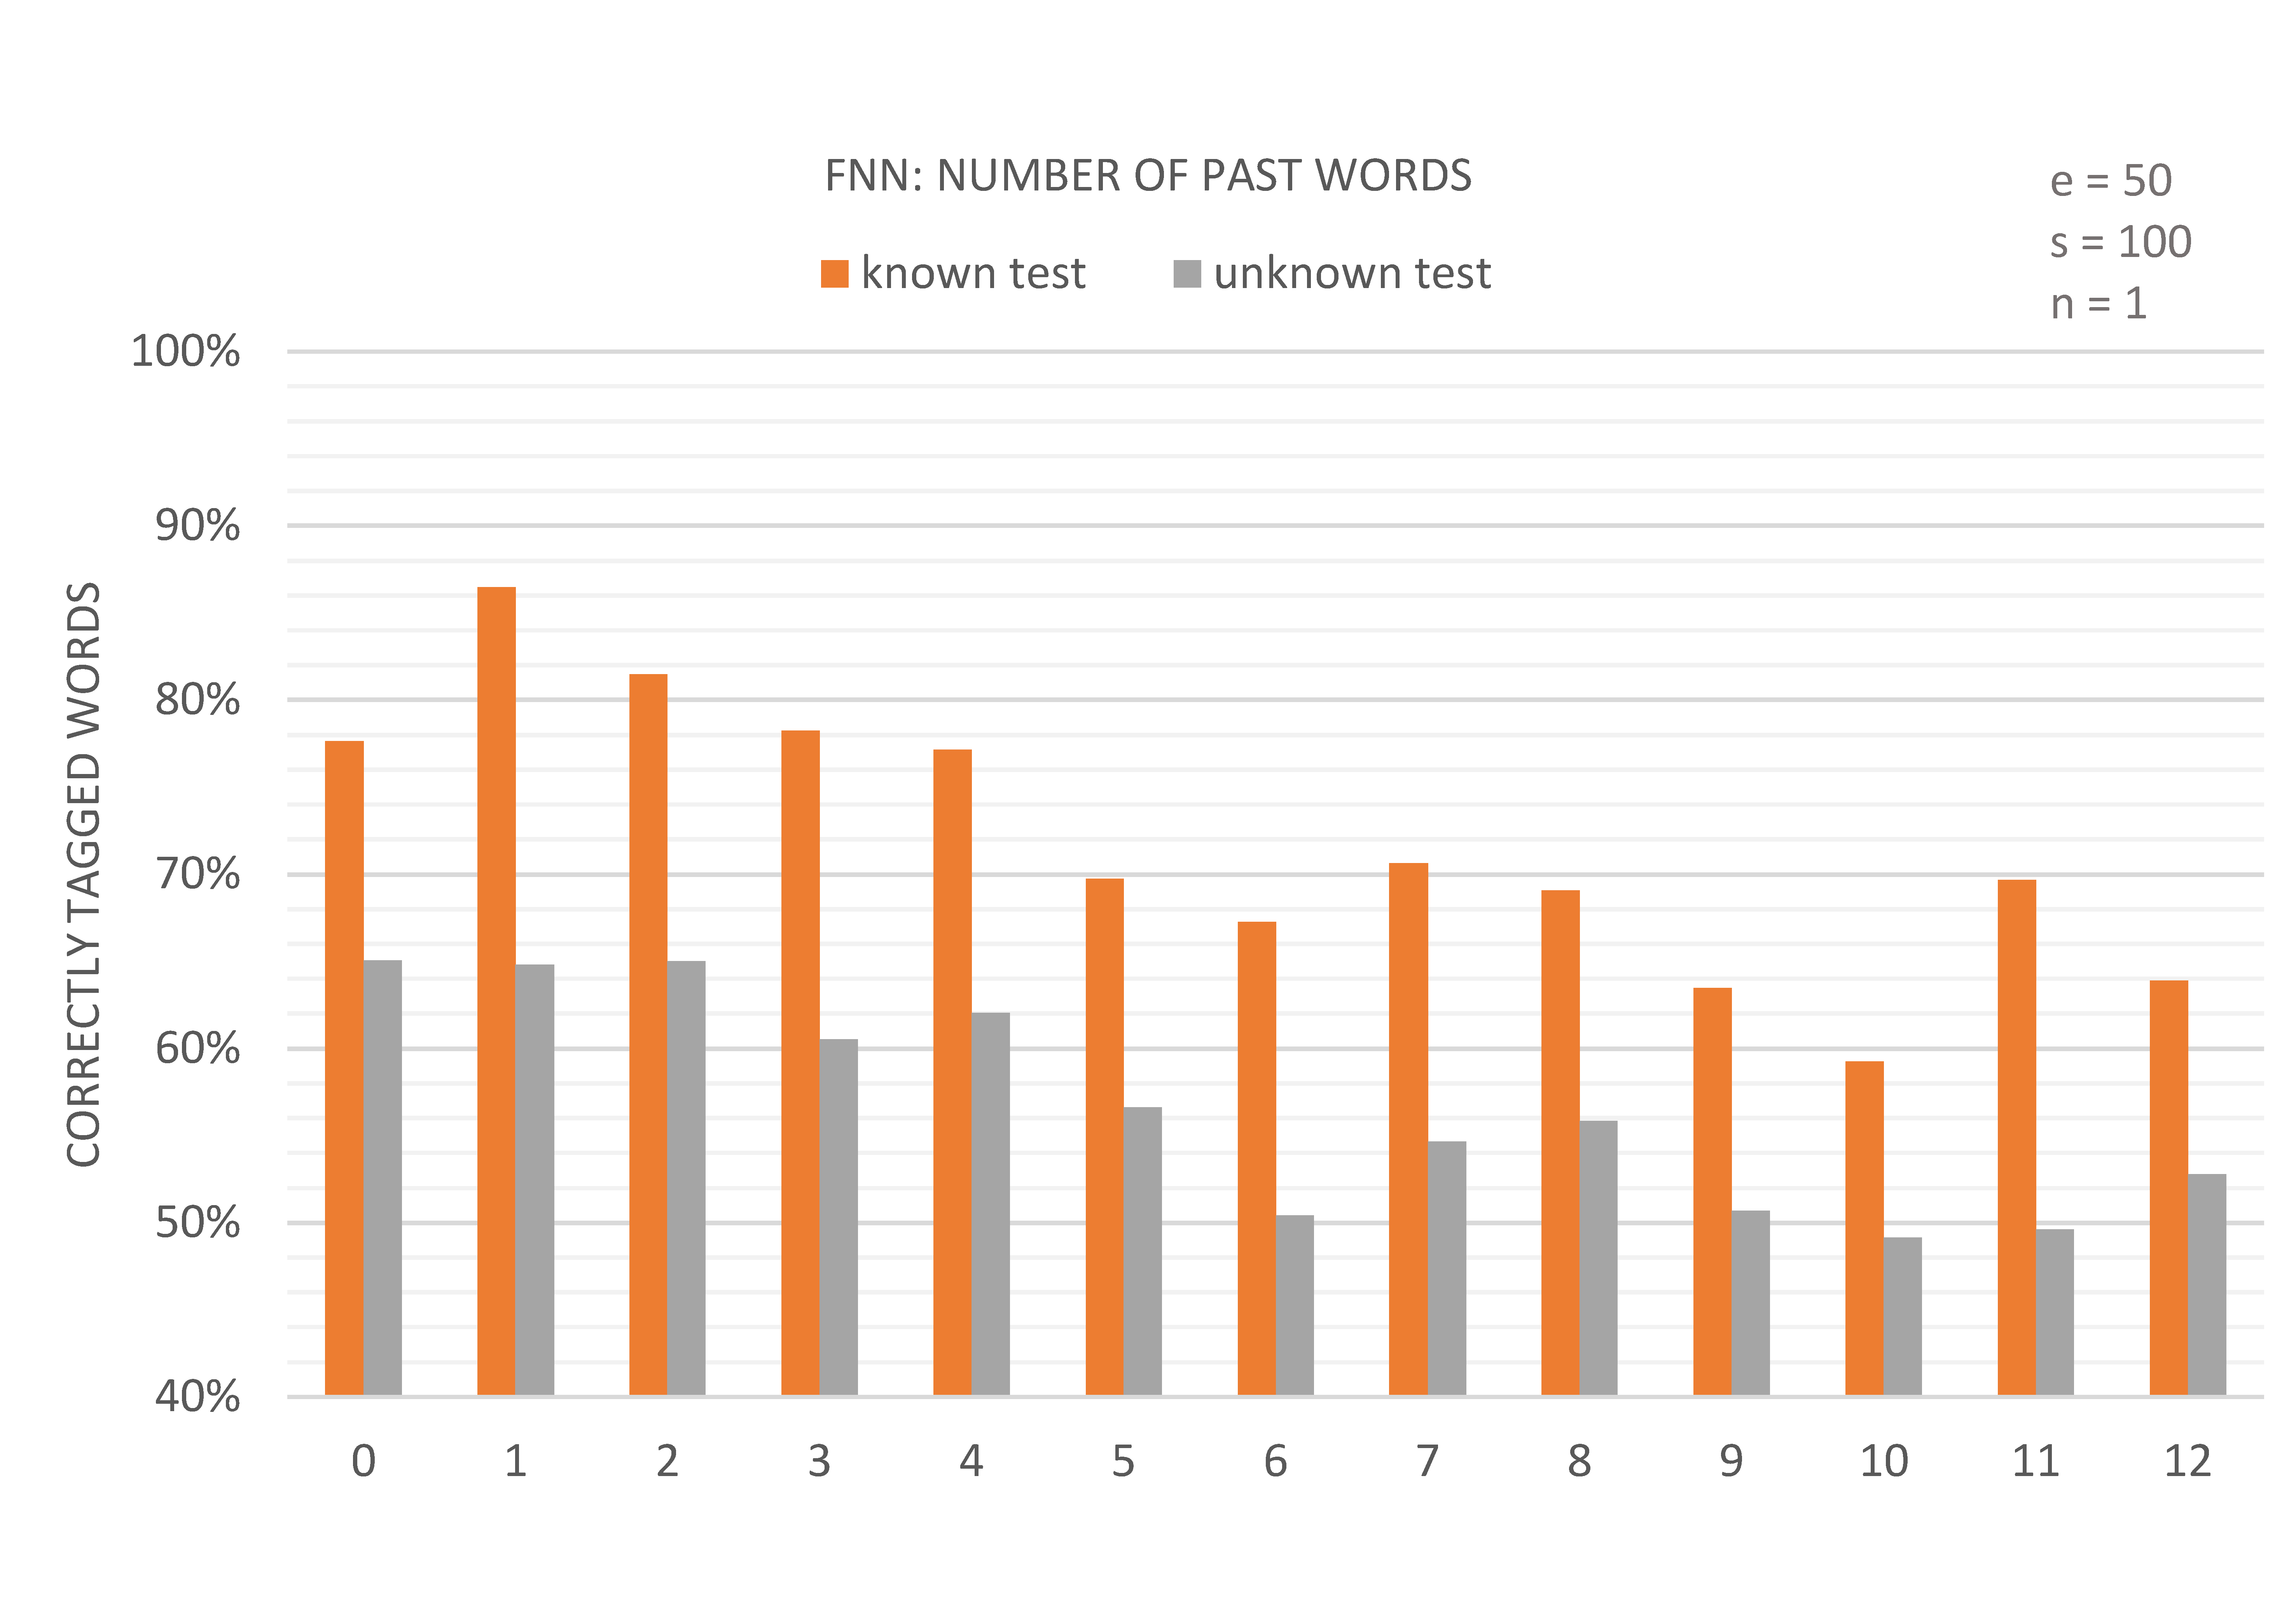
\includegraphics[width=\textwidth]{images/evaluation_fnn_p}
	\caption[FNN Evaluation: Number of Past Words]{The evaluation results of the FNN for parameter \tt{p}: the number of preceding words. Number of correctly tagged words in percent.}
	\label{f.evaluation.fnn.p}
\end{figure}

\begin{figure}[H]
	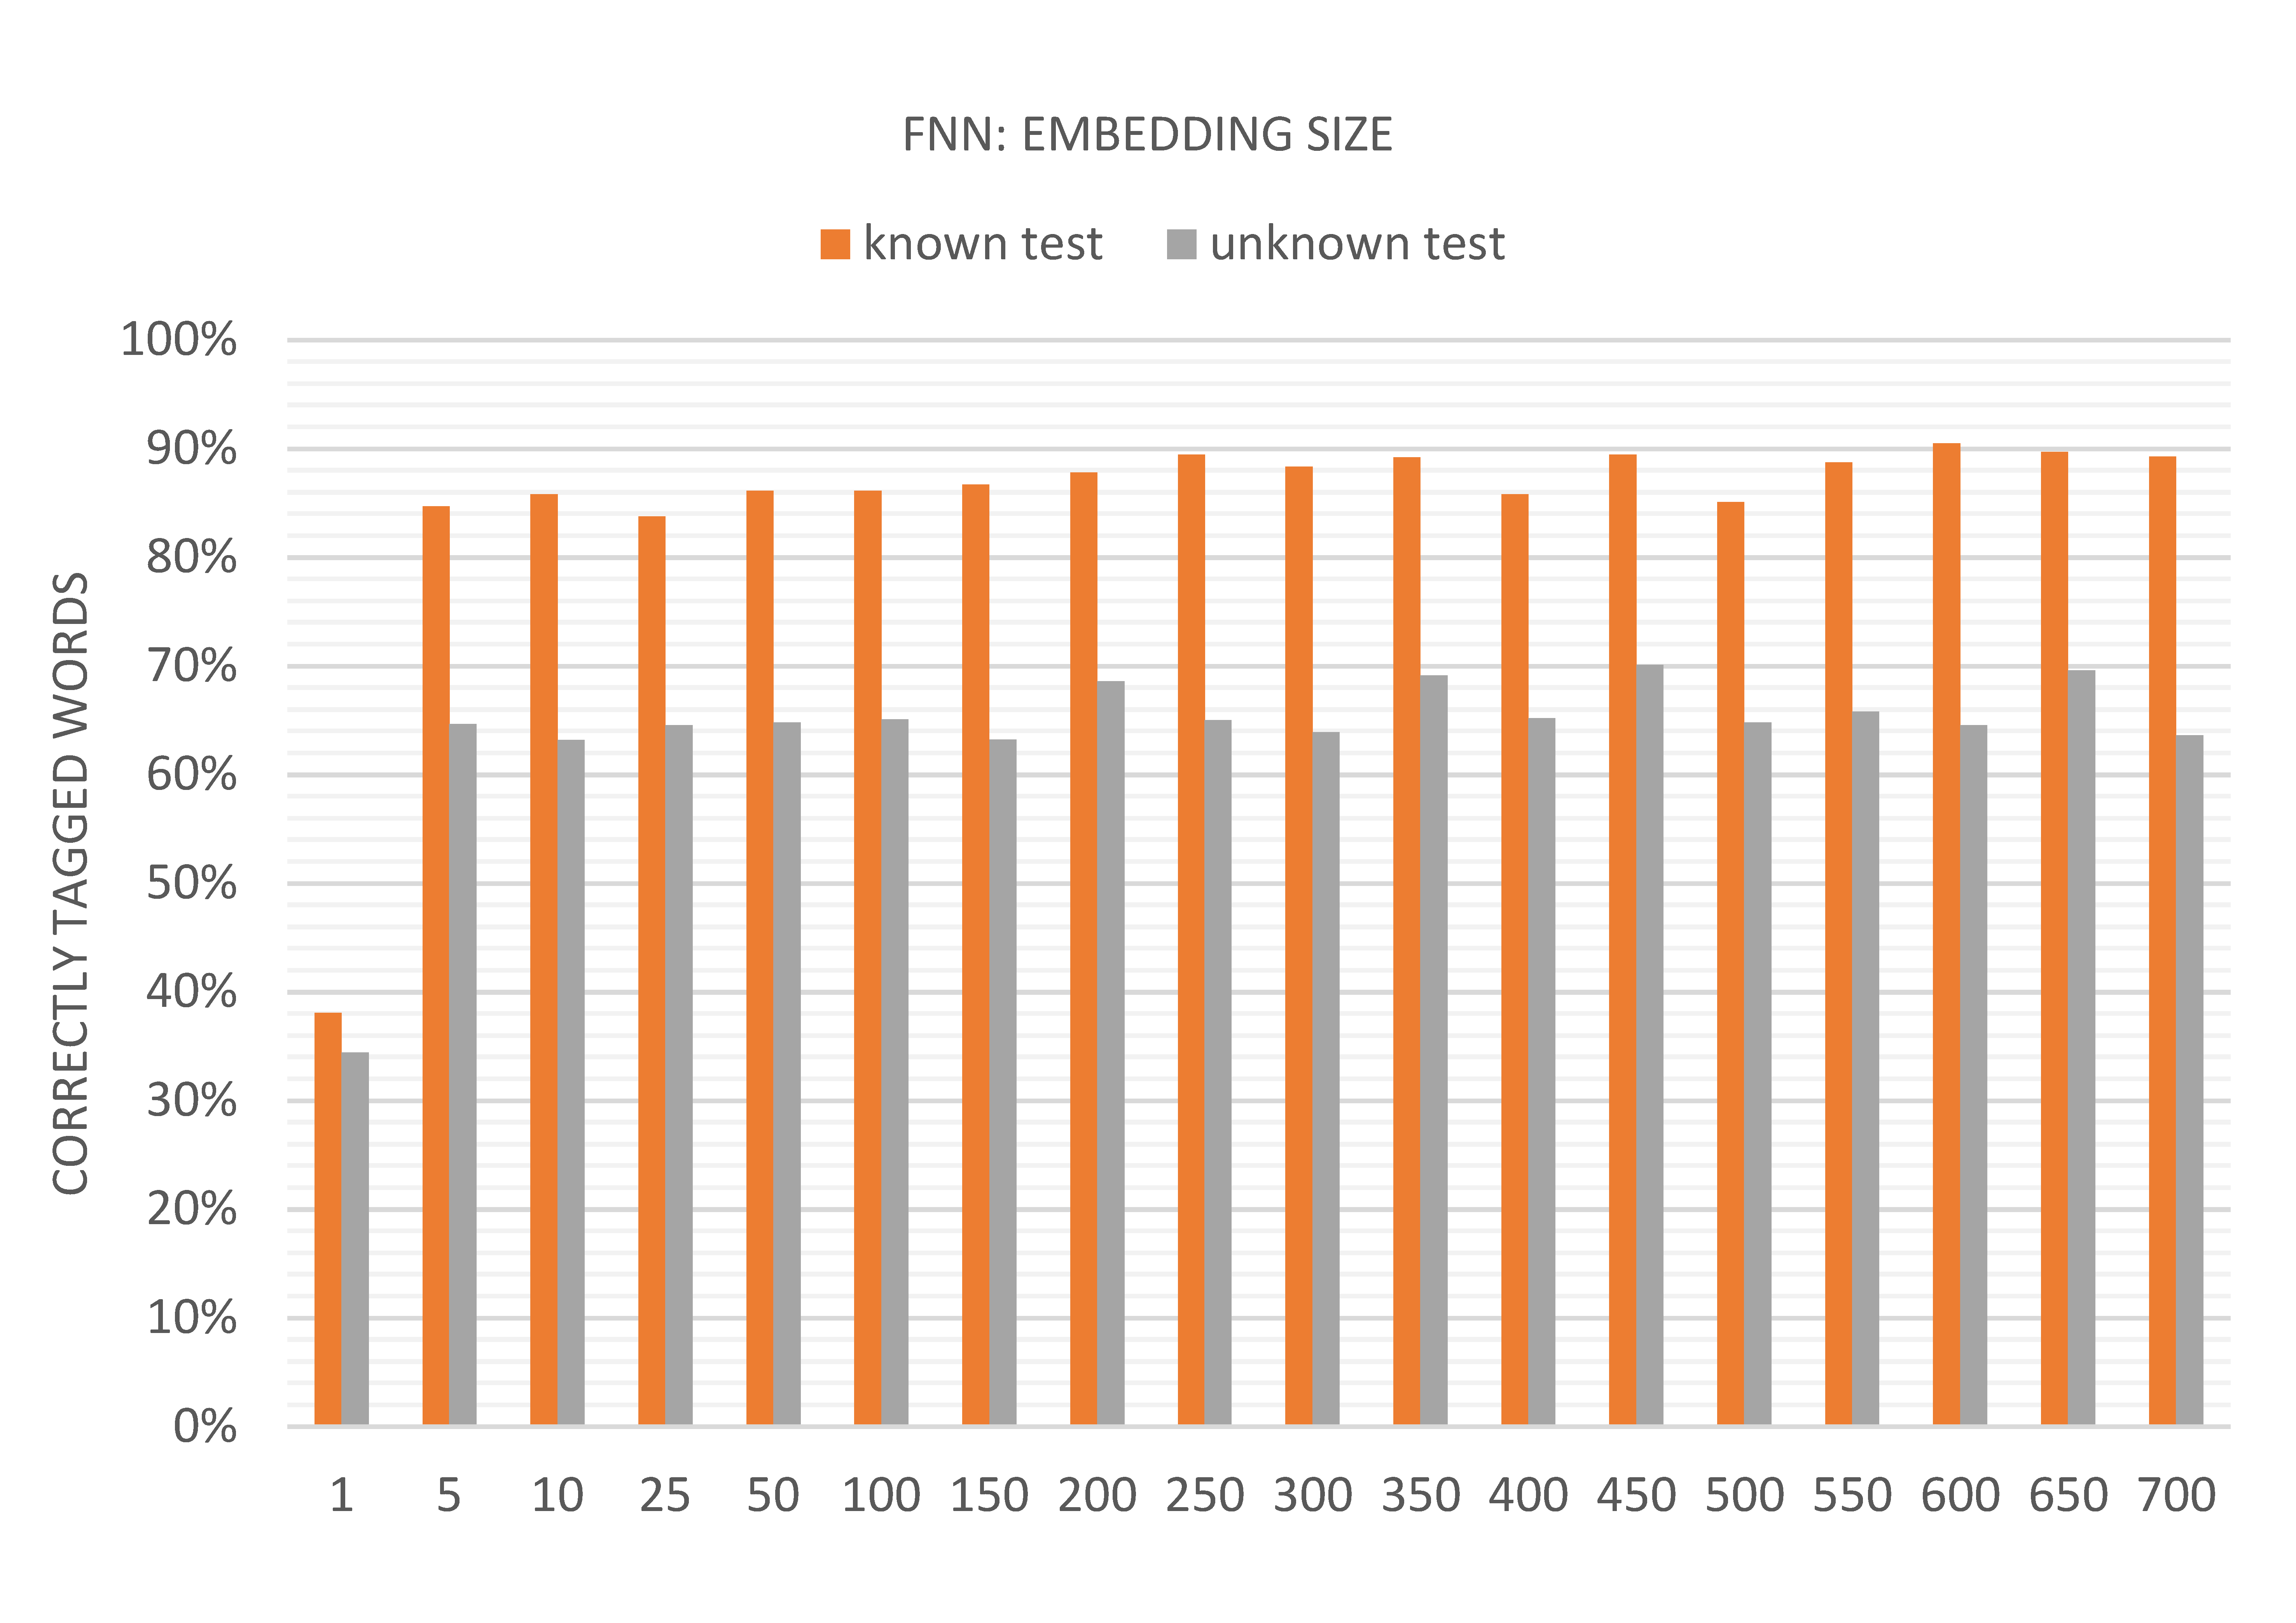
\includegraphics[width=\textwidth]{images/evaluation_fnn_e}
	\caption[FNN Evaluation: Number of Past Words]{The evaluation results of the FNN for parameter \tt{e}: the embedding size. Number of correctly tagged words in percent.}
	\label{f.evaluation.fnn.e}
\end{figure}

\begin{figure}[H]
	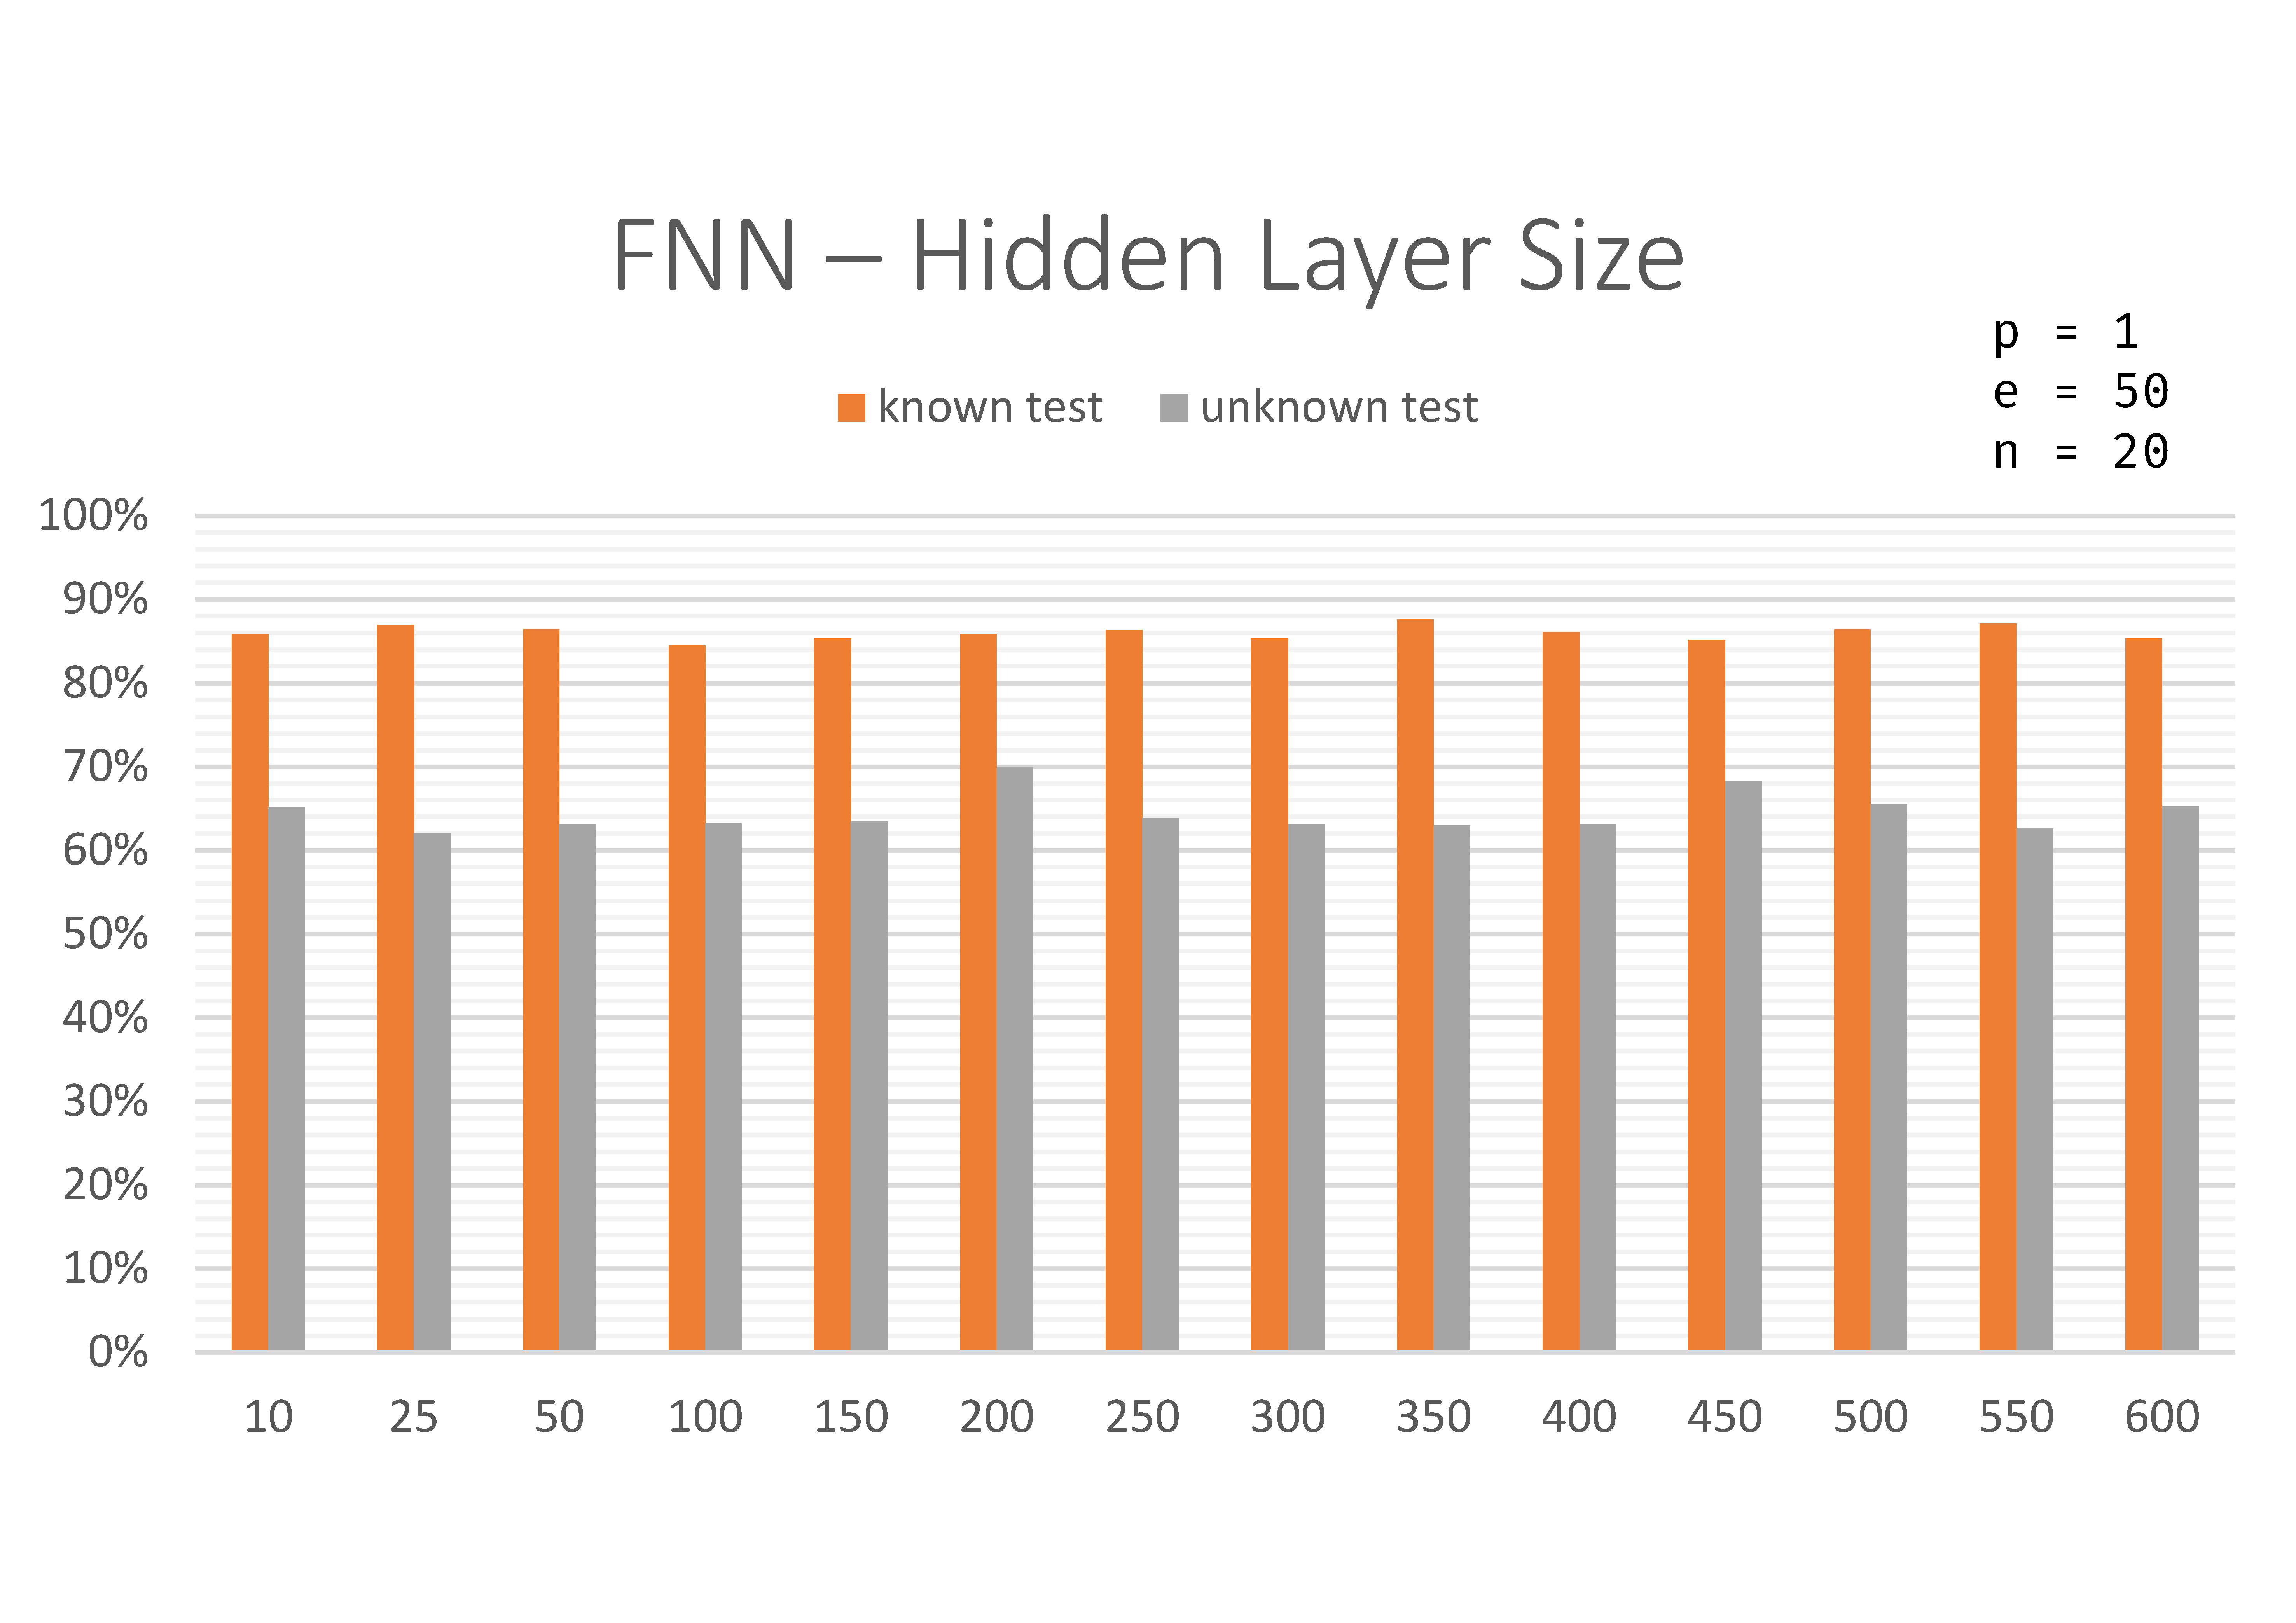
\includegraphics[width=\textwidth]{images/evaluation_fnn_s}
	\caption[FNN Evaluation: Hidden Layer Size]{The evaluation results of the FNN for parameter \tt{s}: the size of the hidden layer. Number of correctly tagged words in percent.}
	\label{f.evaluation.fnn.s}
\end{figure}

\begin{figure}[H]
	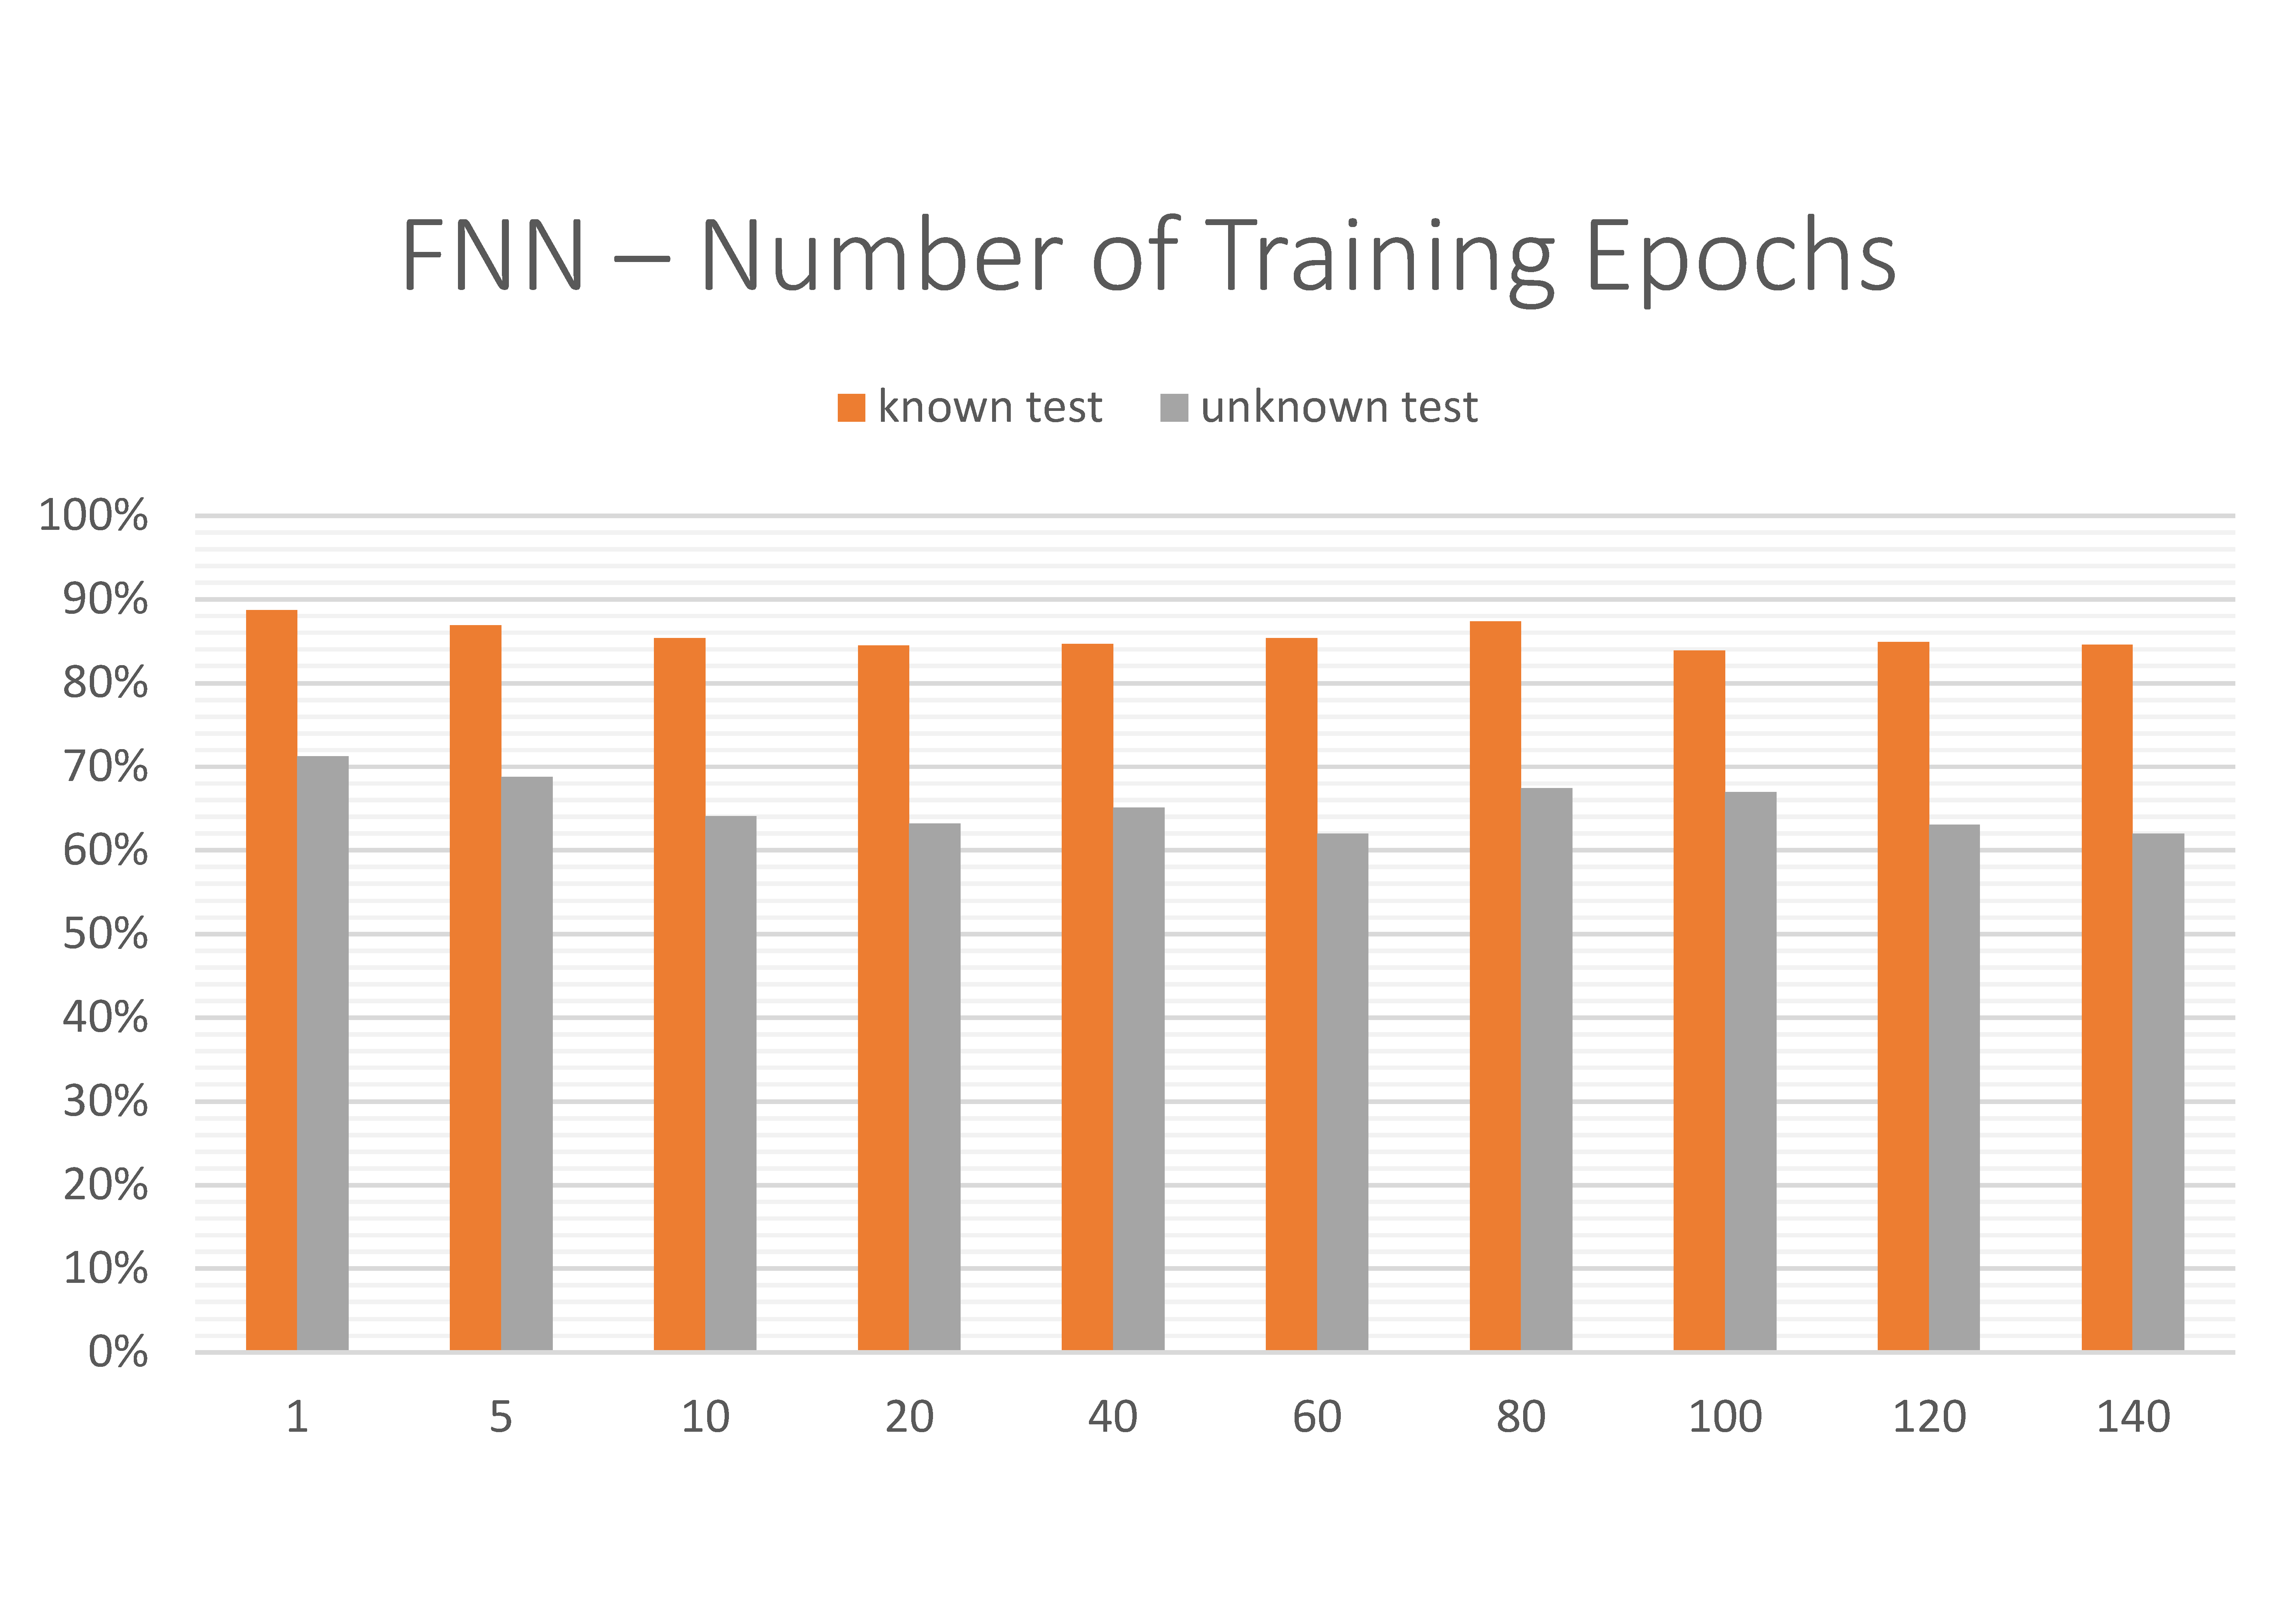
\includegraphics[width=\textwidth]{images/evaluation_fnn_n}
	\caption[FNN Evaluation: Number of Training Epochs]{The evaluation results of the FNN for parameter \tt{n}: the number of training epochs. Number of correctly tagged words in percent.}
	\label{f.evaluation.fnn.n}
\end{figure}

\subsection{Recurrent Neural Network Models}\label{c.evaluation.results.rnn}
...

\subsection{Hidden Markov Models}\label{c.evaluation.results.hmm}
After evaluating the neural network based language models, the HMM is evaluated in the following. For this purpose, the previous HMM which was trained on the basis of the training data generated by T. Michael \cite{michael2016} is compared to a new HMM trained on the basis of the training data proposed in this thesis. The evaluation was carried out using the known and the unknown test; the results are presented in figure \ref{f.evaluation.hmm}.

\begin{figure}[H]
	\centering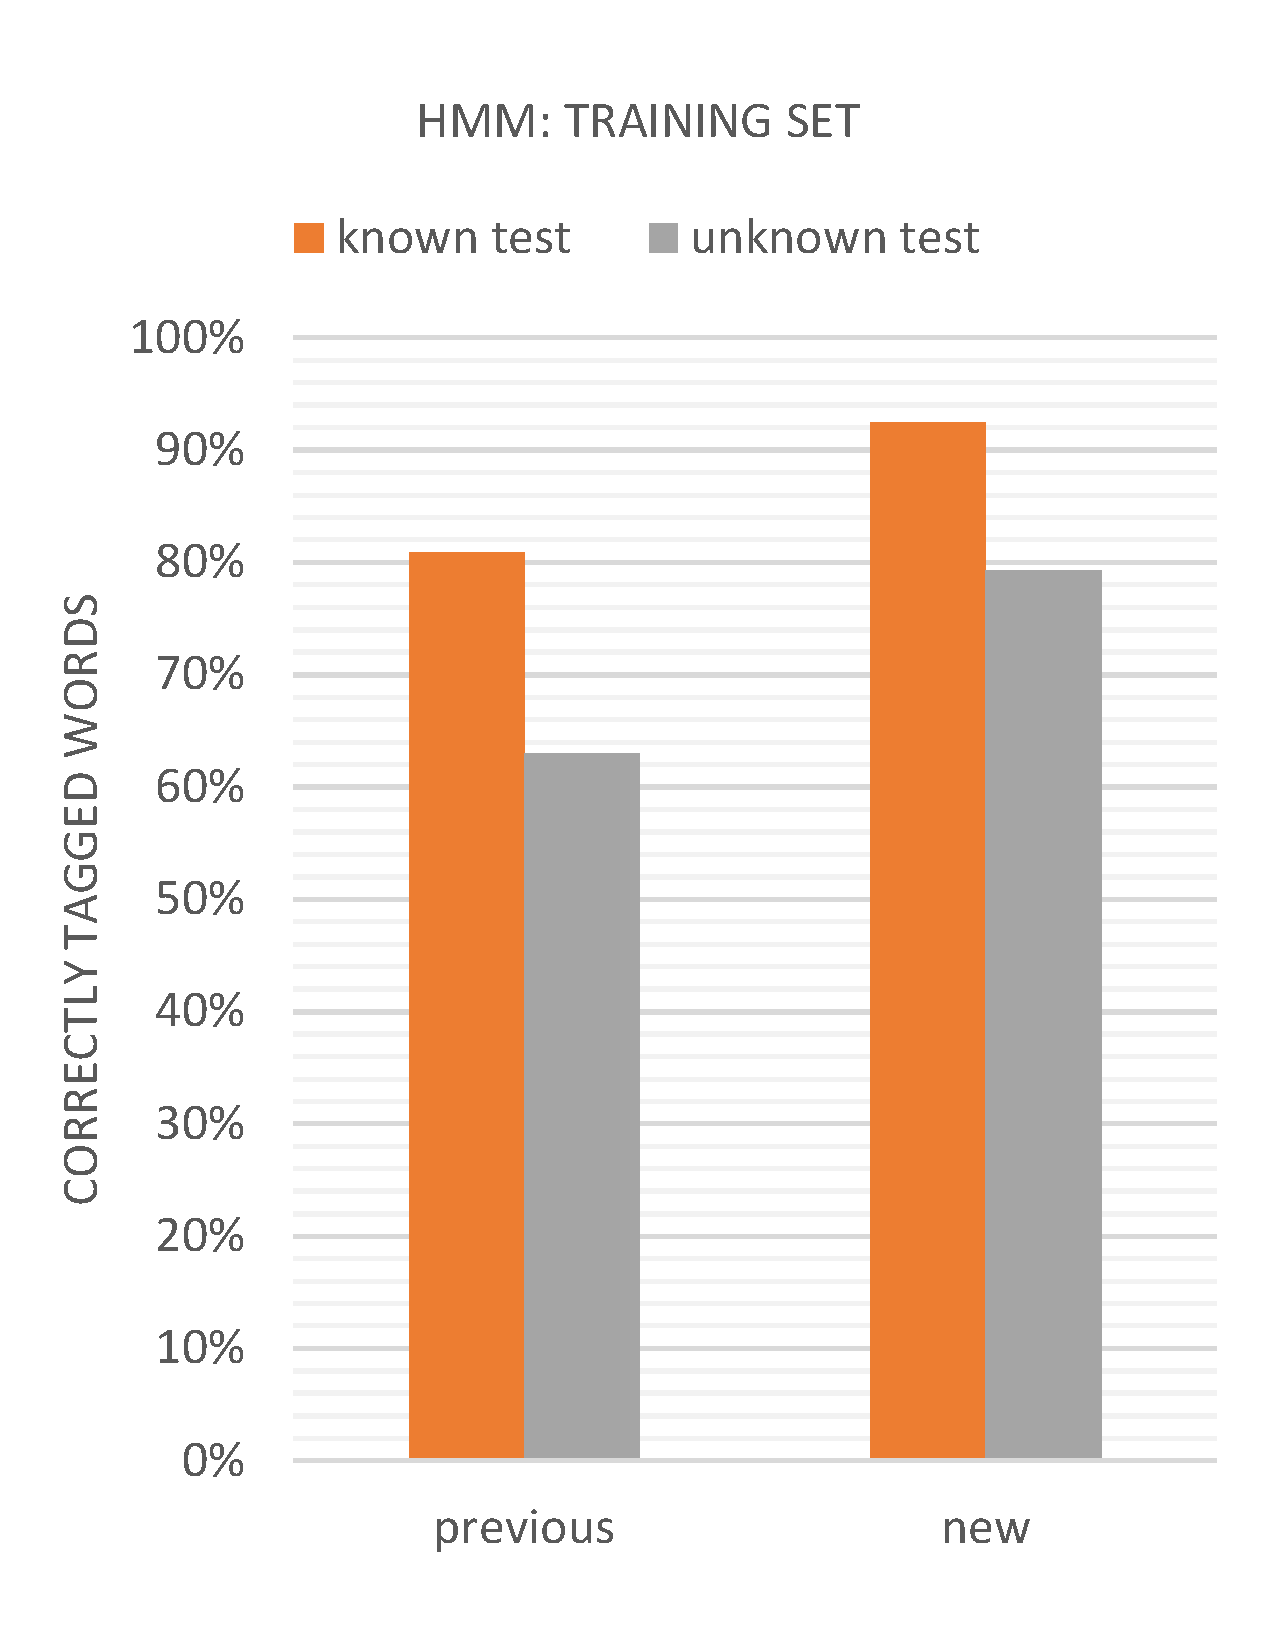
\includegraphics[width=.7\textwidth]{images/evaluation_hmm}
	\caption[HMM Evaluation]{The evaluation results of the previous HMM trained by T. Michael \cite{michael2016} and the new HMM based on the new training data proposed in this thesis.}
	\label{f.evaluation.hmm}
\end{figure}

The previous HMM tagged \tt{82.5\%} of the words of the known test and \tt{63.0\%} of the unknown test correctly, whereas it was \tt{93.4\%} for the known and \tt{79.3\%} for the unknown test for the new HMM. It was evident that the HMM, which was based on the new training data, performed significantly better than the previous HMM. Especially the result for the unknown test is remarkable, as the accuracy increases by more than \tt{16\%}.

It should be noted that the comparison of the previous and the new HMM model based on the known test has some limitations, as the known test was not fully known\footnote{As described in chapter \ref{c.evaluation.test}, the known test contains \tt{584} sentences. \tt{375} sentences are included in he corpus of the previous HMM, resulting in \tt{35.8\%} of the sentences of the known test, that were completely unknown to the previous HMM.} to the previous HMM. Nevertheless, the major part of the known test set was based on training templates that were already used to build the corpus for the previous HMM, which is why it still scored well with more than 4 correct tags out of 5.

\section{Overall Comparison}\label{c.evaluation.comparison}
...

% ===================================================================================
\chapter{Discussion and Conclusion}\label{c.conclusion}
The final chapter summarizes the work of this thesis and the evaluation results achieved. It discusses the evaluation findings and reveals potential areas for further research based on the knowledge gained in this thesis.

\section{Summary}\label{c.conclusion.summary}
The aim to develop a neural network based part-of-speech tagger for the advisory Artificial Conversational Agent \Alex\ was accomplished within the scope of this thesis.

A tagger module was implemented featuring a feed-forward neural network as well as a recurrent neural network. A training corpus containing tagged sentences was created with the help of an improved set of sentence templates. With both neural network architectures, various language models were trained on this corpus using parameter variation. These models were then evaluated with two corresponding tests sets, containing sentences from the training corpus (known data) and unknown sentences.

\section{Discussion}\label{c.conclusion.discussion}
...

\section{Future work}\label{c.conclusion.future}
Although a high accuracy of the language models was achieved with an improved training corpus and the neural network approaches used in this thesis, further research could be done in certain areas to fine-tune and improve the templates as well as the tagging results.

As demonstrated in the preceding chapters, the methodology used in this thesis was found to be appropriate for an initial exploration into improving the tagging results. Going forward, however, there are certain areas and components of the methodology that could be optimized, which will be outlined in the following.

Rather than manually deleting training templates that contain a lot of useless combinations of data from the database, an additional module could check these combinations automatically in advance. Depending on the query result of such a data validation module, the generated training sentence would then be included or excluded from the training corpus. This way, the general sentence templates can still be used knowing that meaningless training sentences will not be considered.

In this thesis, parameters that were thought to influence the tagging results, such as the number of previous words, the size of the hidden layer, the size of the word embeddings and the number of training epochs were analyzed. Yet there are additional parameters, which could also be examined to improve the accuracy further. For the FNN, parameters of possible interest are the number of subsequent words (in addition to the number of previous words), the number of hidden layers, the type of the activation function for the neurons and the training optimizer. The use of word embeddings with a particular embedding size for the RNN could be interesting too, as well as the type of the activation function and the optimizer, which are possible additional parameters. Moreover, an exponential decay for the learning rate of the optimizer, especially for the RNN, could be explored.

Another potential way to improve the tagging accuracy, could be to use pretrained instead of randomly initialized word embeddings in the training process. This is a relevant direction to explore, as it was previously shown that word embeddings that were trained on large German text corpora contain a high level of syntactical and semantical information \cite{mueller2015}.

Furthermore, to improve the evaluation process, it could be extended with a more fine-grained output concerning semantical topics such as degrees, locations, persons or module titles. This way, a statement could be made about how well the model performs on each topic and if there are significant differences between the evaluation results. This knowledge could then be used to systematically improve the training templates.

All in all, this thesis has demonstrated several ways of improving the tagger, which is not only of importance for the scope of this thesis and \Alex\ but which can also be used as a starting point for improving other chatbots, or systems that use a POS tagger in general.

% ===================================================================================
\bibliographystyle{plain}
\bibliography{bibliography}

% ===================================================================================
\appendix
\chapter{Appendix}\label{c.appendix}

\section{Set of sentence templates}\label{c.appendix.sentencetemplates}
\lstinputlisting[language=plain, label={l.trainingtemplate}]{listings/training_template.txt}

\end{document}